
%! program = pdflatex

\documentclass[12pt]{article}
\usepackage{amsmath}
\usepackage{natbib}
\usepackage{graphicx}
\usepackage{amssymb}
\usepackage{epstopdf}
\usepackage{float} % to keep the figures in place

\usepackage{color}
\newcommand{\cred}{ \color{red}}
\newcommand{\cgreen}{\color{green}}
\newcommand{\cblue}{\color{blue}}
\newcommand{\cmag}{\color{magenta}}
\newcommand{\bn}{\begin{enumerate}}
\newcommand{\en}{\end{enumerate}}
\newcommand{\bi}{\begin{itemize}}
\newcommand{\ei}{\end{itemize}}
\newcommand{\be}{\begin{eqnarray}}
\newcommand{\ee}{\end{eqnarray}}
\newcommand{\by}{\begin{eqnarray*}}
\newcommand{\ey}{\end{eqnarray*}}
\renewcommand{\labelenumi}{(\alph{enumi}) }
%
\usepackage[margin=2.2cm, includehead]{geometry}% see geometry.pdf on how to lay out the page. There's lots.
\geometry{letterpaper} % or letter or a5paper or ... etc
% \geometry{landscape} % rotated page geometry
%\bibpunct{(}{)}{;}{a}{,}{,}
%\setlength{\textwidth}{16cm}
%\setlength{\textheight}{21cm}
\def\nonumber{\global\@eqnswfalse}
\newcounter{parnum}
\newcommand{\N}{%
  \noindent\refstepcounter{parnum}%
   \makebox[\parindent][l]{\textbf{[\arabic{parnum}]}}\quad  }
% Use a generous paragraph indent so numbers can be fit inside the
% indentation space.
\setlength{\parindent}{1.5em}

% See the ``Article customise'' template for come common customisations

\date{}
%\date{} % delete this line to display the current date

%%% BEGIN DOCUMENT
\usepackage{Sweave}
\begin{document}
\Sconcordance{concordance:HW3.tex:HW3.Rnw:%
1 47 1 1 0 25 1 1 8 1 2 4 1 2 2 3 1 1 4 3 1 1 4 13 1 1 2 1 0 2 1 4 0 1 %
2 2 1 1 2 1 0 1 1 1 2 8 0 1 1 7 0 1 2 4 1 1 2 1 0 1 1 4 0 1 2 2 1 1 2 7 %
0 1 2 2 1 1 2 5 0 1 2 3 1 1 7 4 0 1 2 5 1 1 2 1 0 1 1 4 0 1 2 13 1 1 2 %
1 0 3 1 4 0 1 2 1 1 1 2 1 0 1 1 4 0 1 2 1 1 1 2 8 0 1 1 6 0 1 2 2 1 1 2 %
1 0 1 1 4 0 1 2 2 1 1 2 7 0 1 2 2 1 1 2 5 0 1 2 8 1 1 2 1 0 1 1 4 0 1 2 %
11 1 1 7 1 2 14 1 1 2 1 0 2 1 4 0 1 2 2 1 1 2 1 0 1 1 4 0 1 2 1 1 1 2 8 %
0 1 1 6 0 1 2 4 1 1 2 1 0 1 1 4 0 1 2 2 1 1 2 7 0 1 2 2 1 1 2 5 0 1 2 3 %
1 1 7 4 0 1 2 5 1 1 2 1 0 1 1 4 0 1 2 10 1 1 2 1 0 2 1 8 0 5 1 4 0 1 2 %
11 1 1 2 1 0 1 1 23 0 1 2 1 1 1 2 1 0 1 1 6 0 1 2 1 8 4 0 1 2 4 1 1 2 1 %
0 1 1 4 0 1 2 5 1 1 2 1 0 2 1 4 0 1 2 6 1 1 2 1 0 1 1 4 0 1 2 6 1 1 2 1 %
0 1 1 4 0 1 2 11 1 1 3 1 0 2 1 23 0 1 2 3 1 1 2 1 0 1 1 6 0 1 2 1 8 4 0 %
1 2 5 1 1 2 1 0 1 1 4 0 1 2 6 1 1 2 1 0 2 1 4 0 1 2 6 1 1 2 1 0 1 1 4 0 %
1 2 6 1 1 2 1 0 1 1 4 0 1 2 14 1 1 2 1 0 1 3 25 0 1 2 4 1 1 2 1 0 1 1 6 %
0 1 2 4 1 1 2 1 0 1 1 4 0 1 2 5 1 1 2 1 0 2 1 4 0 1 2 4 1 1 2 1 0 1 1 4 %
0 1 2 4 1 1 2 1 0 1 1 4 0 1 2 15 1 1 2 1 0 1 3 27 0 1 2 4 1 1 2 1 0 1 1 %
6 0 1 2 1 10 4 0 1 2 5 1 1 2 1 0 1 1 4 0 1 2 5 1 1 2 1 0 1 1 4 0 1 2 6 %
1 1 2 1 0 1 1 4 0 1 2 66 1}

%\large
%\maketitle
\newtheorem{thm}{Theorem}[section]
\newtheorem{cor}[thm]{Corollary}
\newtheorem{lem}[thm]{Lemma}
\newtheorem{prop}[thm]{Proposition}
\newtheorem{defn}[thm]{Definition}
\newtheorem{exam}[thm]{Example}
\newtheorem{qstn}[thm]{Question}

%%%
\newpage
\begin{center}
{\bf Homework 3 - STAT 511}\\
Amal Agarwal
\end{center}
%==========================
\section*{Answer 1}
\bn
\item
Let us call y as the stopping distance (response variable) and x as the speed (predictor variable). For Exploratory Data Analysis (EDA) following scatter plots were obtained:
\begin{itemize}
\item Plot of y vs. x
\begin{figure}[H]
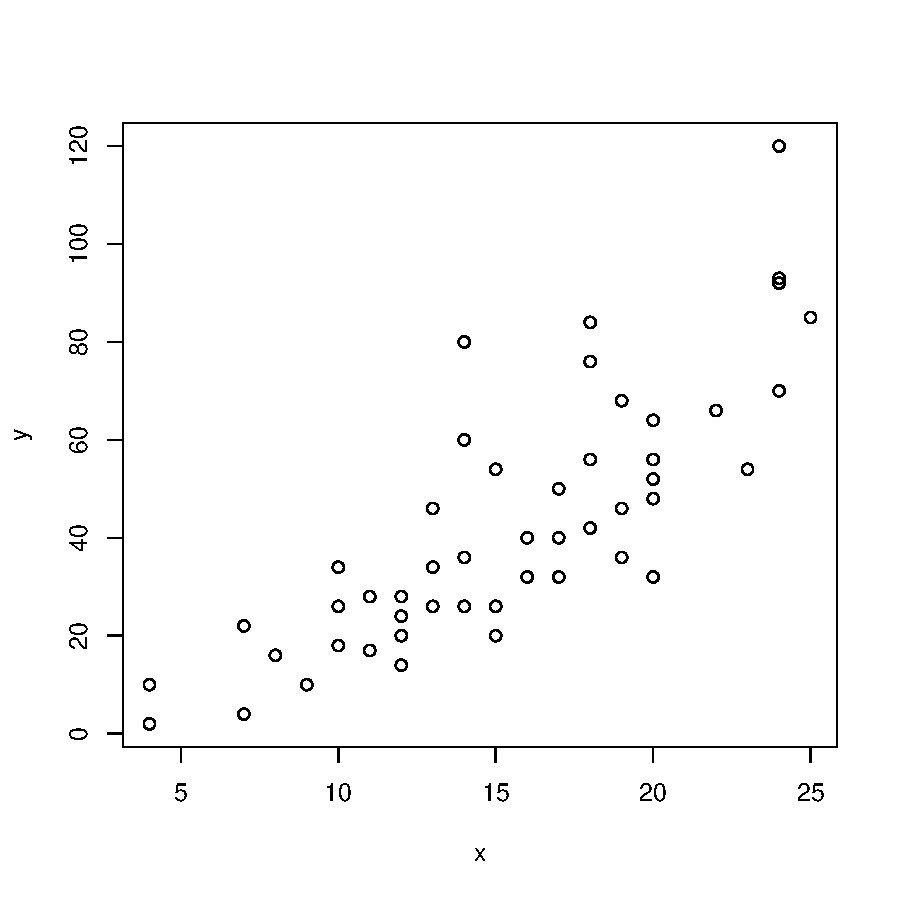
\includegraphics{HW3-001}
\end{figure}
\clearpage

\item Plot of $\sqrt{y}$ vs. x
\begin{figure}[H]
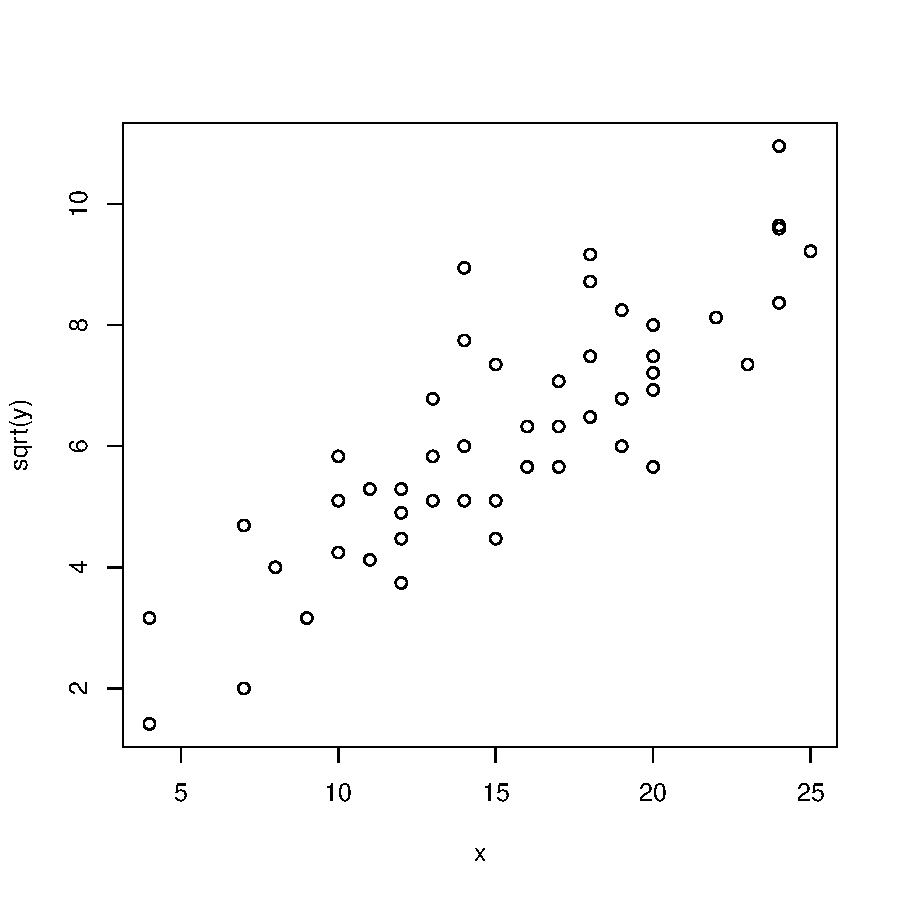
\includegraphics{HW3-002}
\end{figure}

%\item Plot of $y$ vs. $x^2$
\begin{figure}[H]
\end{figure}

%\item Plot of $log(y)$ vs. x
\begin{figure}[H]
\end{figure}
\end{itemize}
It can be observed that the scatter plot of $y$ vs. $x$ indicates a non linear relationship between $y$ and $x$. Further tha density of data points for $x<7$ and $x>21$ is relatively lower than for $8<x<20$. The transformations $log(y)$ vs. $x$ can be ruled out since it does not look linear. The transformation $y$ vs. $x^2$ looks promising in terms of fitting a simple linear model. But, the scatter plot that shows the most closest linear relationship after the transformation is $\sqrt{y}$ vs. x. Note: The transformations that didn't seem to work are not shown explicitly in the form of  scatter plots.
\item
The simple linear regression model in R that can be used to fit the given data is 
\begin{equation*}
\begin{aligned}
y &= \beta_0 + \beta_1 x + \epsilon
\end{aligned}
\end{equation*}
where $\epsilon \sim N(0,\sigma^2)$

\item Using lm in R, to estimate model parameters and residuals.
\begin{figure}[H]
\begin{Schunk}
\begin{Sinput}
> fit1=lm(y~x)
> plot(x,y)
> abline(fit1)
\end{Sinput}
\end{Schunk}
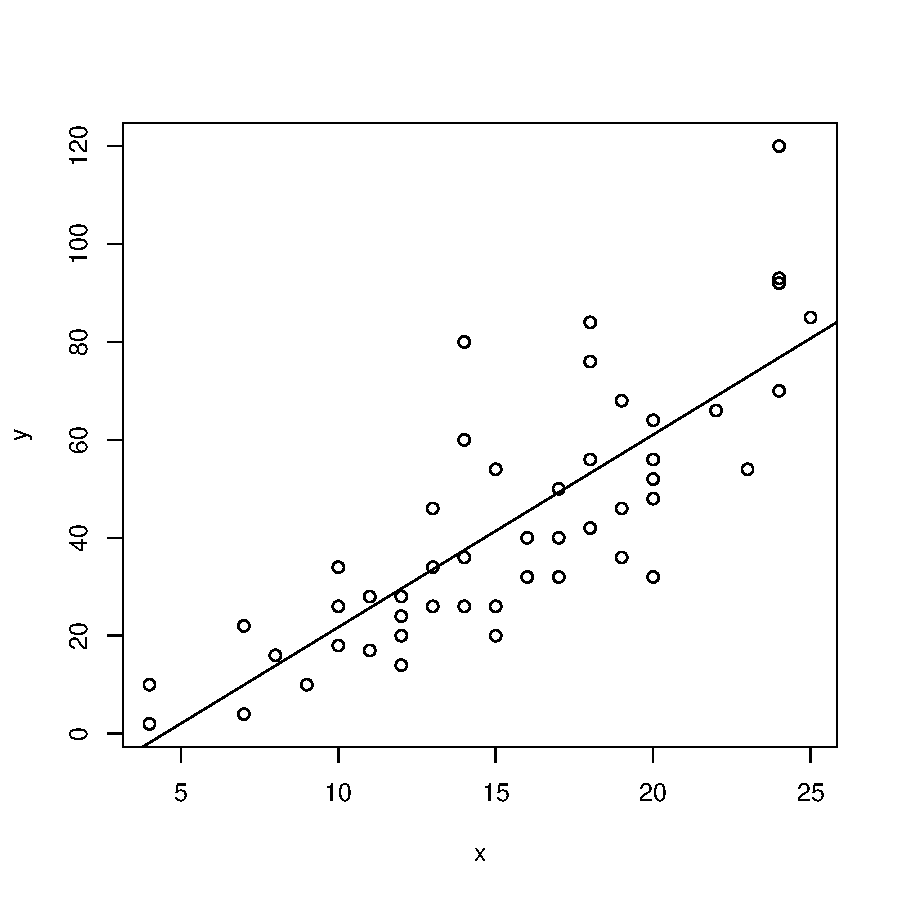
\includegraphics{HW3-005}
\end{figure}

\begin{figure}[H]
\begin{Schunk}
\begin{Sinput}
> residuals=fit1$resid
> hist(residuals)
> ## the table given in summary(fit)
> summary(fit1)$coef
\end{Sinput}
\begin{Soutput}
              Estimate Std. Error   t value     Pr(>|t|)
(Intercept) -17.579095  6.7584402 -2.601058 1.231882e-02
x             3.932409  0.4155128  9.463990 1.489836e-12
\end{Soutput}
\begin{Sinput}
> summary(fit1)$sigma
\end{Sinput}
\begin{Soutput}
[1] 15.37959
\end{Soutput}
\end{Schunk}
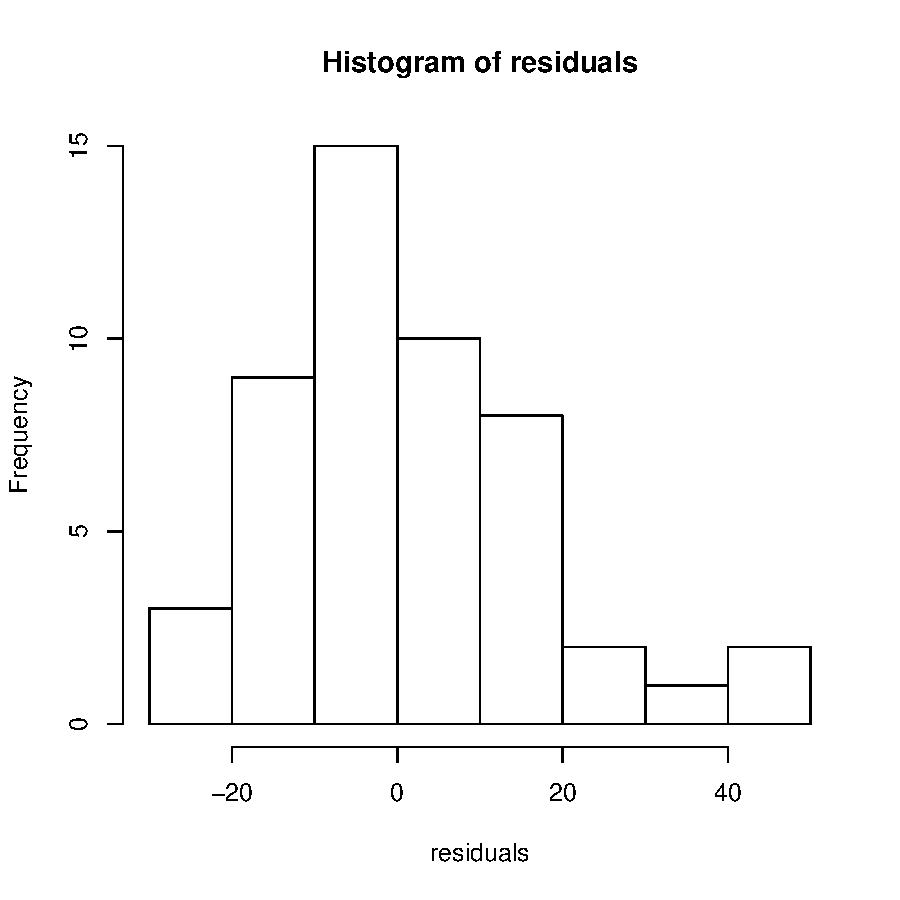
\includegraphics{HW3-006}
\end{figure}
\clearpage

\item
\begin{figure}[H]
\begin{Schunk}
\begin{Sinput}
> yhat=fit1$fitted.values
> plot(yhat,y)
\end{Sinput}
\end{Schunk}
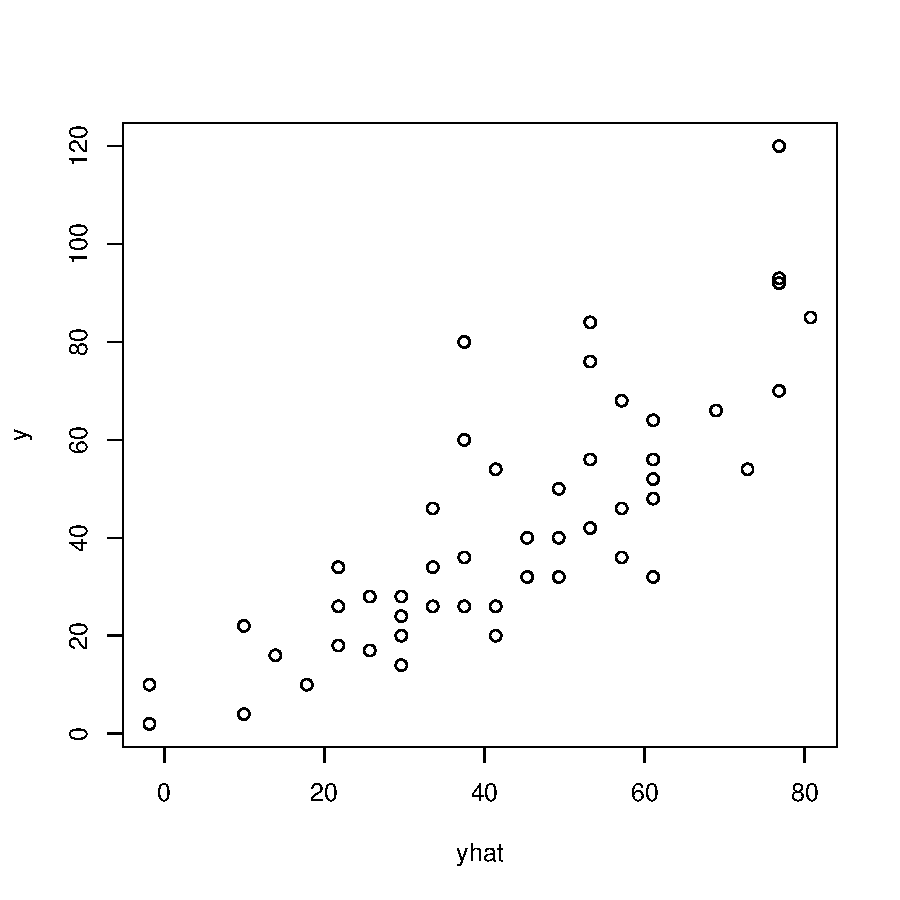
\includegraphics{HW3-007}
\end{figure}

The mean of the residuals is given as
\begin{Schunk}
\begin{Sinput}
> mean(residuals)
\end{Sinput}
\begin{Soutput}
[1] 8.65974e-17
\end{Soutput}
\end{Schunk}
This is very close to zero which indicates that our assumption of $E(\epsilon)=0$ is satisfied.
To check for homoscedasticity, residuals can be plotted against x as
\begin{figure}[H]
\begin{Schunk}
\begin{Sinput}
> plot(x,residuals)
\end{Sinput}
\end{Schunk}
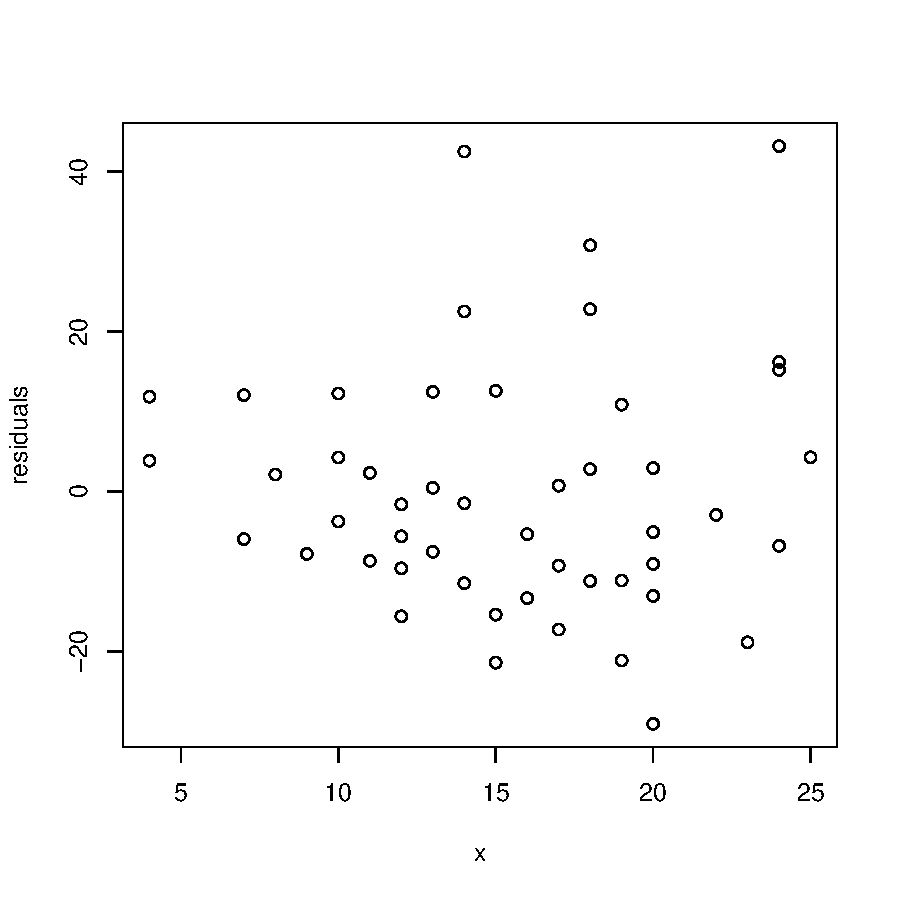
\includegraphics{HW3-009}
\end{figure}
Clearly, as x increases, the fluctuations of residuals around zero increases which implies that the estimated variance of the residuals increase with the covariate "speed". This funnel shaped behaviour is called heteroscedascity which clearly violates our assumption of homoscedascity in the classical linear model. 

The column rank of the design matrix X can be calculated as:
\begin{Schunk}
\begin{Soutput}
[1] 2
\end{Soutput}
\end{Schunk}
which confirms our assumption of full column rank design matrix.

\clearpage
\begin{itemize}
\item QQ Plot for residuals
\begin{figure}[H]
\begin{Schunk}
\begin{Sinput}
> qqnorm(residuals)
> qqline(residuals)
\end{Sinput}
\end{Schunk}
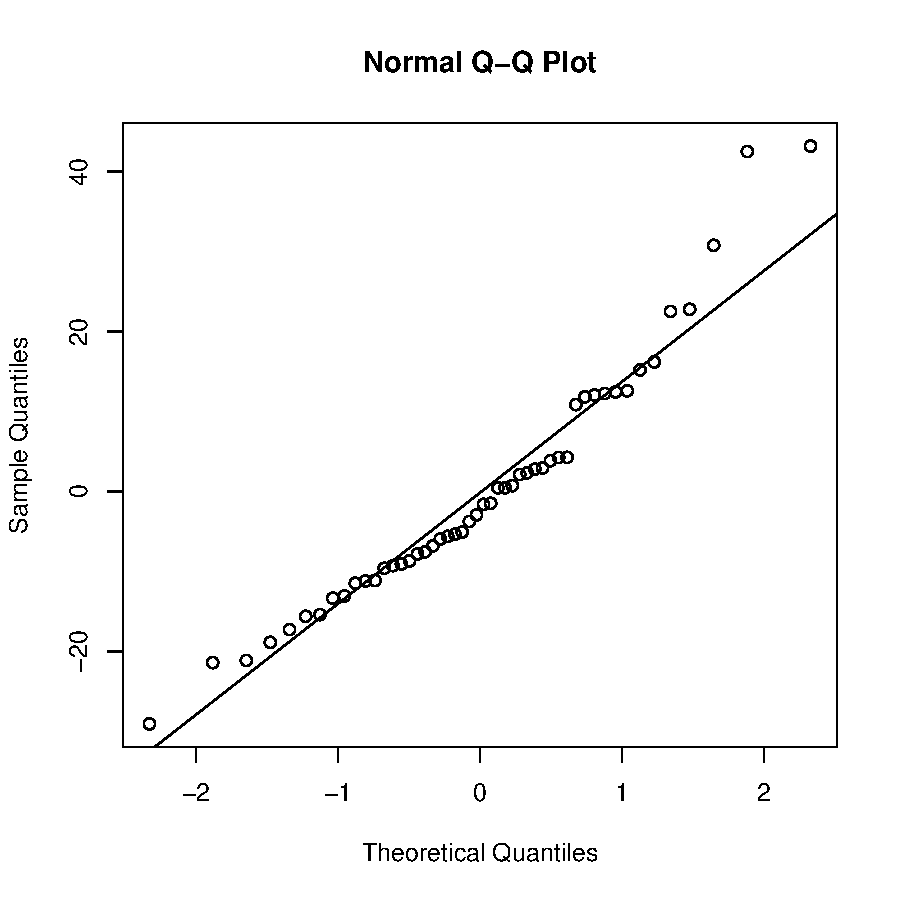
\includegraphics{HW3-011}
\end{figure}
The above QQ plot shows significant deviation from our normality assumption.
\end{itemize}

\item
The modified linear regression model in R that can be used to fit the given data is 
\begin{equation*}
\begin{aligned}
z &= \beta_0 + \beta_1 x + \epsilon
\end{aligned}
\end{equation*}
where $z=\sqrt{y}$ is the transformed response variable. Here we are using the power transform on the response variable as indicated by EDA.
\item Using lm in R, to estimate modified model parameters and residuals.
\begin{figure}[H]
\begin{Schunk}
\begin{Sinput}
> z<-sqrt(y)
> fit2=lm(z~x)
> plot(x,z)
> abline(fit2)
\end{Sinput}
\end{Schunk}
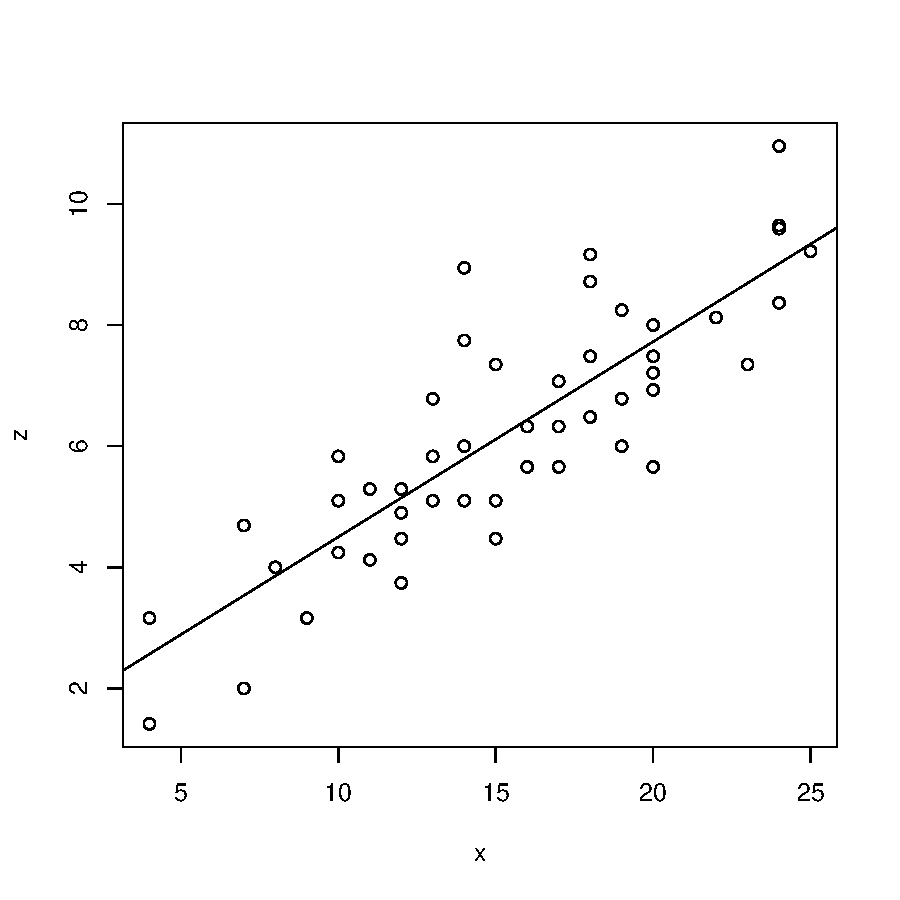
\includegraphics{HW3-012}
\end{figure}
\begin{figure}[H]
\begin{Schunk}
\begin{Sinput}
> residuals.transformed=fit2$resid
> hist(residuals.transformed)
\end{Sinput}
\end{Schunk}
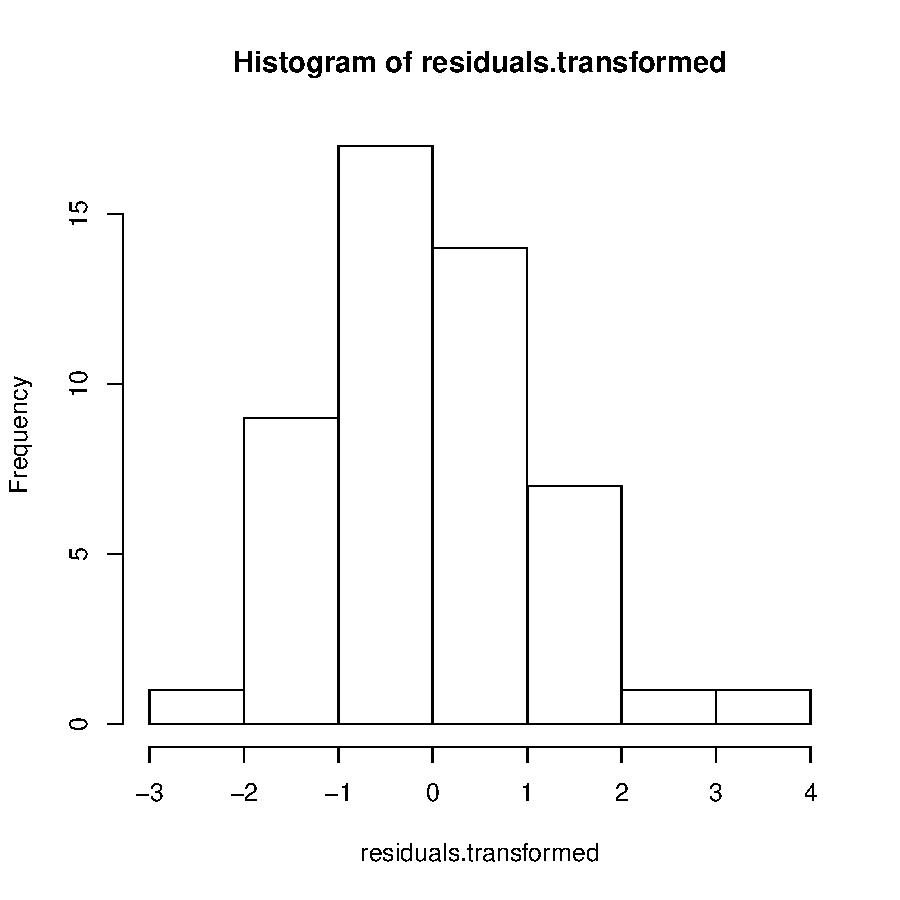
\includegraphics{HW3-013}
\end{figure}

\begin{Schunk}
\begin{Sinput}
> summary(fit2)$coef
\end{Sinput}
\begin{Soutput}
             Estimate Std. Error   t value     Pr(>|t|)
(Intercept) 1.2770502 0.48444202  2.636126 1.126220e-02
x           0.3224125 0.02978377 10.825106 1.773141e-14
\end{Soutput}
\begin{Sinput}
> summary(fit2)$sigma
\end{Sinput}
\begin{Soutput}
[1] 1.102402
\end{Soutput}
\end{Schunk}

\clearpage
\begin{figure}[H]
\begin{Schunk}
\begin{Sinput}
> zhat=fit2$fitted.values
> plot(zhat,z)
\end{Sinput}
\end{Schunk}
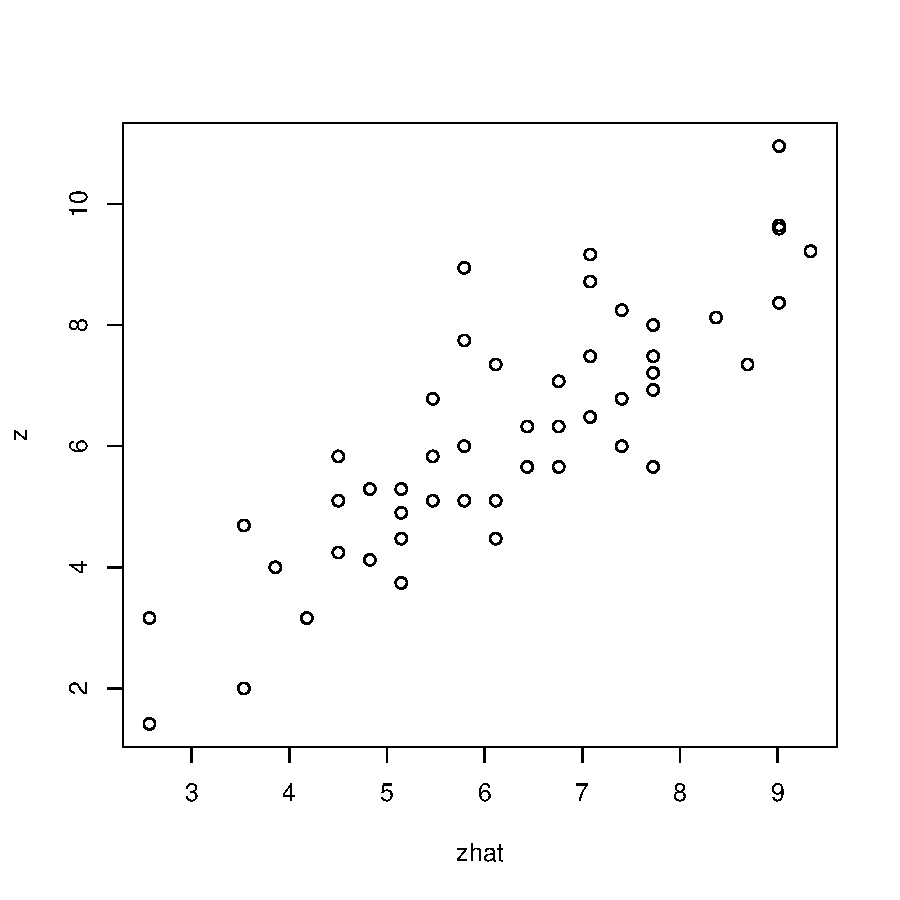
\includegraphics{HW3-015}
\end{figure}

The mean of transformed residuals is given as
\begin{Schunk}
\begin{Sinput}
> mean(residuals.transformed)
\end{Sinput}
\begin{Soutput}
[1] 3.109546e-17
\end{Soutput}
\end{Schunk}
This is again very close to zero which indicates that our assumption of $E(\epsilon)=0$ is satisfied.
To check for homoscedasticity, the transformed residuals can be plotted against x as
\begin{figure}[H]
\begin{Schunk}
\begin{Sinput}
> plot(x,residuals.transformed)
\end{Sinput}
\end{Schunk}
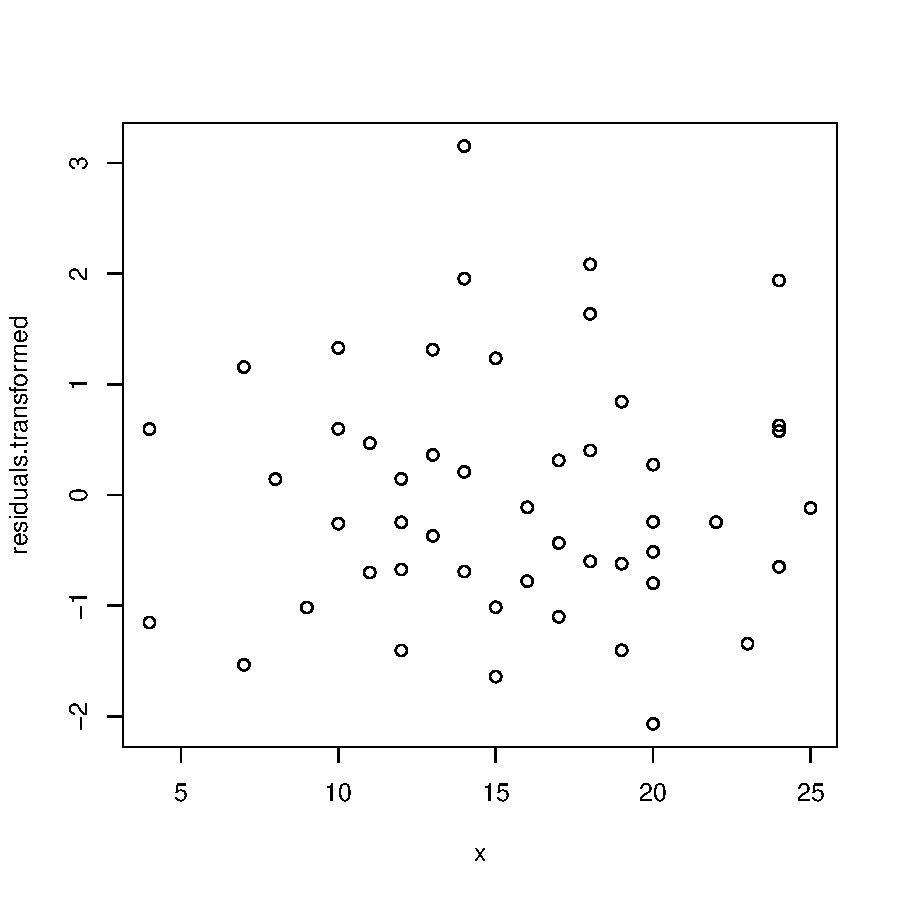
\includegraphics{HW3-017}
\end{figure}
This looks much better since the fluctuations of the transformed residuals around zero is more or less uniform and does not depend on x. Thus our assumption of homoscedascity in the classical linear model is satisfied after the transformation. 
\en
%break
\clearpage

\begin{itemize}
\item QQ Plot for residuals
\begin{figure}[H]
\begin{Schunk}
\begin{Sinput}
> qqnorm(residuals.transformed)
> qqline(residuals.transformed)
\end{Sinput}
\end{Schunk}
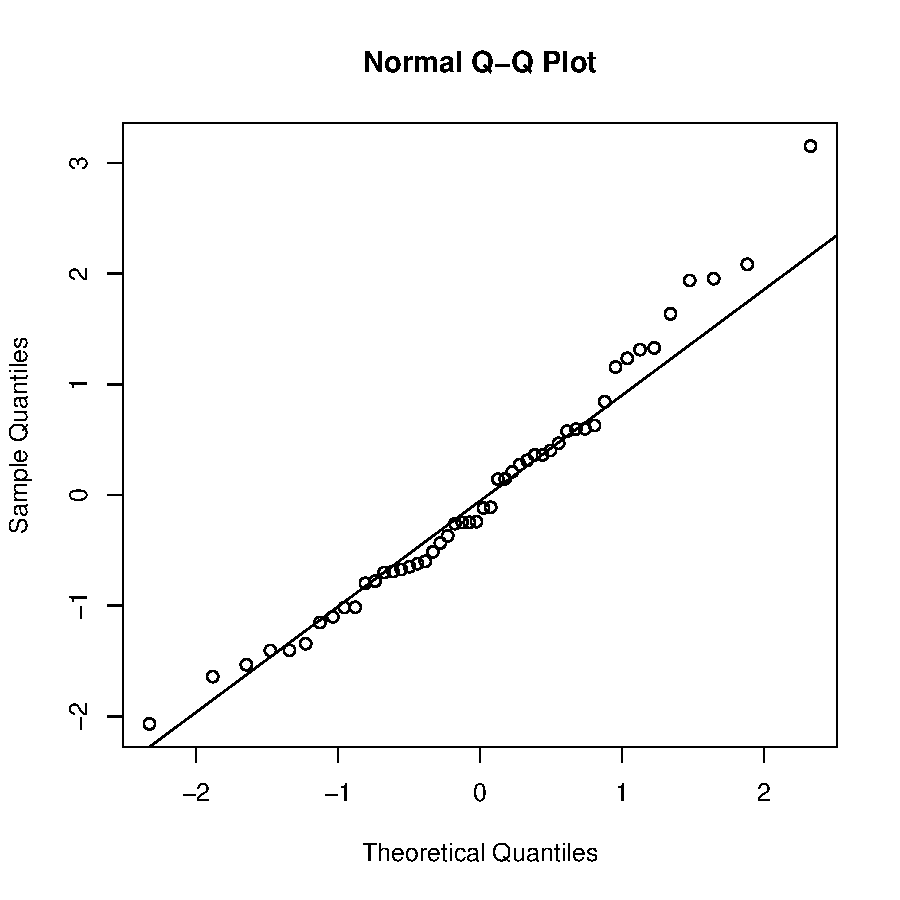
\includegraphics{HW3-018}
\end{figure}
Except for a little fat tail on the right side, the above QQ plot is much better than the previous one. This shows that after transformation, the errors are approximately normally distributed.    
\end{itemize}

\clearpage
\section*{Answer 2}
\bn
\item
Let us call y as the tree girth (response variable) and x as the tree height (predictor variable). For Exploratory Data Analysis (EDA) following scatter plots were obtained:
\begin{itemize}
\item Plot of y vs. x
\begin{figure}[H]
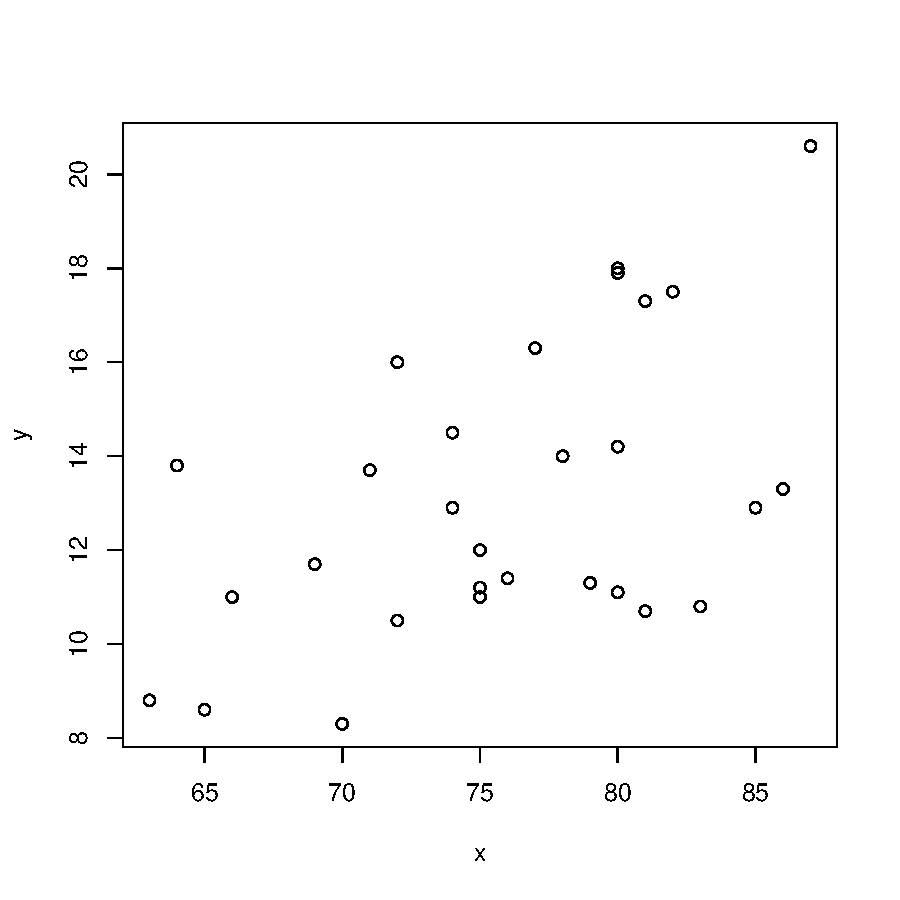
\includegraphics{HW3-019}
\end{figure}
\end{itemize}
It can be observed that the scatter plot of y vs. x doesn't indicate a well defined non linear relationship between y and x. The various power transformations and log transformation also do not help much. Again the scatter plots corresponding to various transformations that don't work, are not shown explicitly.
\item
The simple linear regression model in R that can be used to fit the given data is 
\begin{equation*}
\begin{aligned}
y &= \beta_0 + \beta_1 x + \epsilon
\end{aligned}
\end{equation*}
where $\epsilon \sim N(0,\sigma^2)$ 

\clearpage
\item Using lm in R, to estimate model parameters and residuals.
\begin{figure}[H]
\begin{Schunk}
\begin{Sinput}
> fit1=lm(y~x)
> plot(x,y)
> abline(fit1)
\end{Sinput}
\end{Schunk}
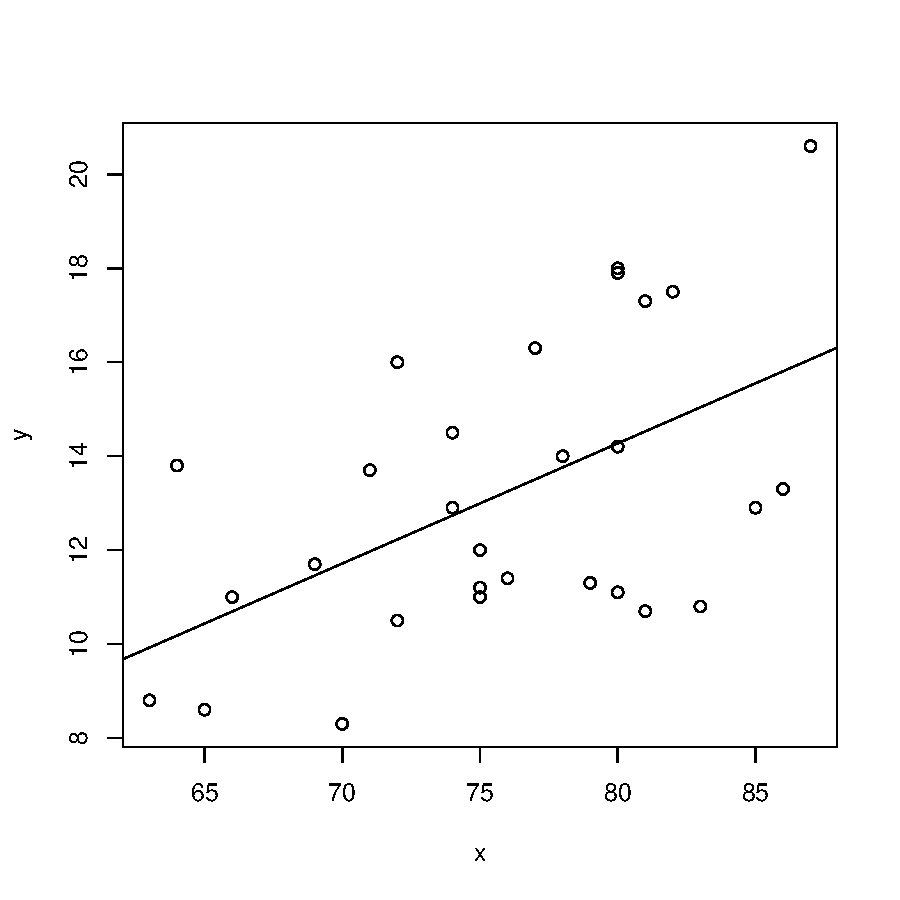
\includegraphics{HW3-020}
\end{figure}

\begin{figure}[H]
\begin{Schunk}
\begin{Sinput}
> residuals=fit1$resid
> hist(residuals)
\end{Sinput}
\end{Schunk}
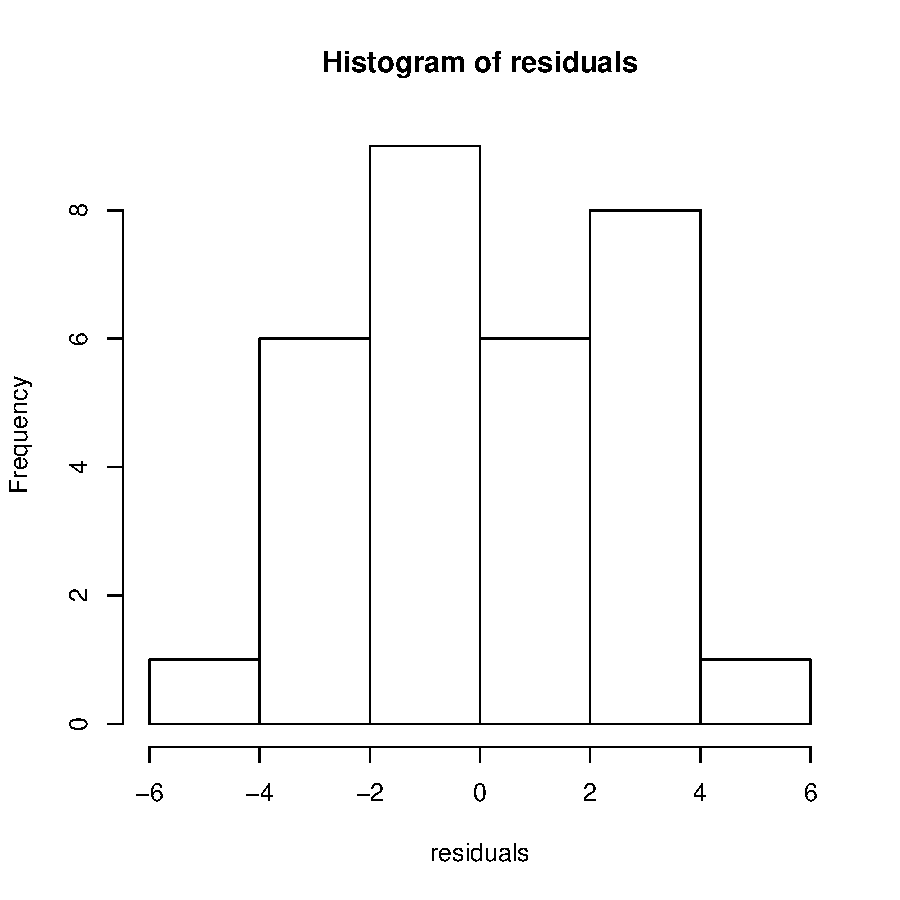
\includegraphics{HW3-021}
\end{figure}

\begin{Schunk}
\begin{Sinput}
> summary(fit1)$coef
\end{Sinput}
\begin{Soutput}
              Estimate Std. Error   t value    Pr(>|t|)
(Intercept) -6.1883945  5.9601994 -1.038286 0.307716768
x            0.2557471  0.0781583  3.272169 0.002757815
\end{Soutput}
\begin{Sinput}
> summary(fit1)$sigma
\end{Sinput}
\begin{Soutput}
[1] 2.727713
\end{Soutput}
\end{Schunk}

\clearpage

\item
\begin{figure}[H]
\begin{Schunk}
\begin{Sinput}
> yhat=fit1$fitted.values
> plot(yhat,y)
\end{Sinput}
\end{Schunk}
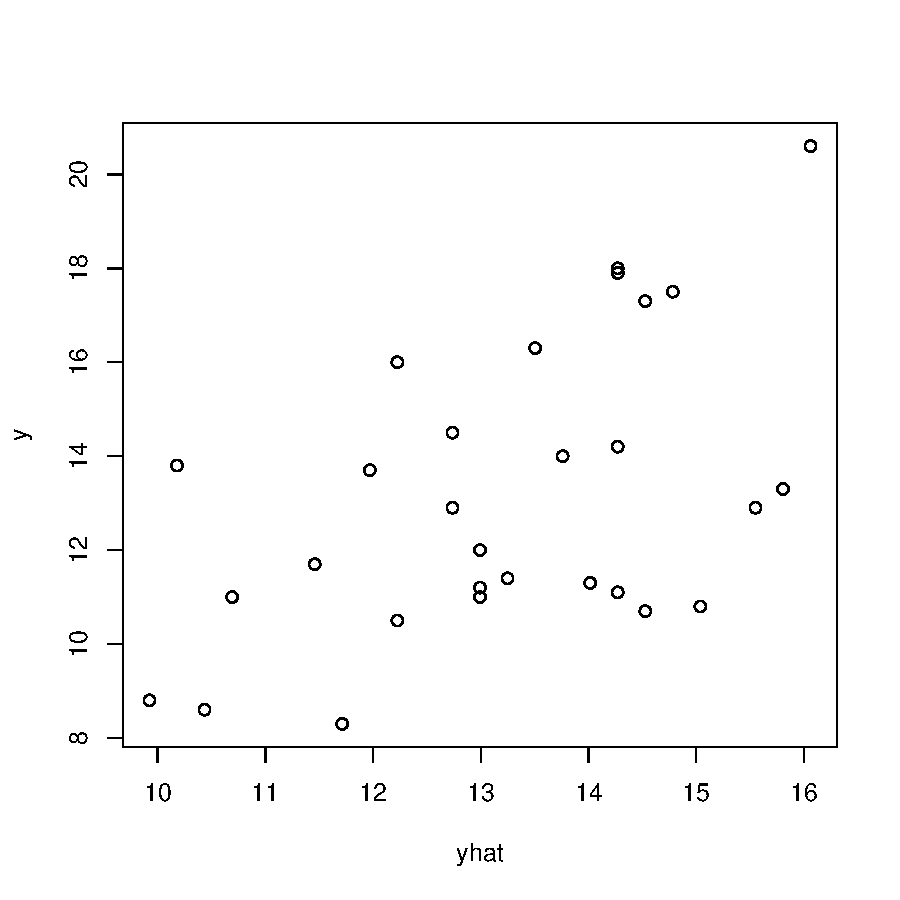
\includegraphics{HW3-023}
\end{figure}

The mean of residuals is given as
\begin{Schunk}
\begin{Sinput}
> mean(residuals)
\end{Sinput}
\begin{Soutput}
[1] -3.192451e-17
\end{Soutput}
\end{Schunk}
This is very close to zero which indicates that our assumption of $E(\epsilon)=0$ is satisfied.
To check for homoscedasticity, residuals can be plotted against x as
\begin{figure}[H]
\begin{Schunk}
\begin{Sinput}
> plot(x,residuals)
\end{Sinput}
\end{Schunk}
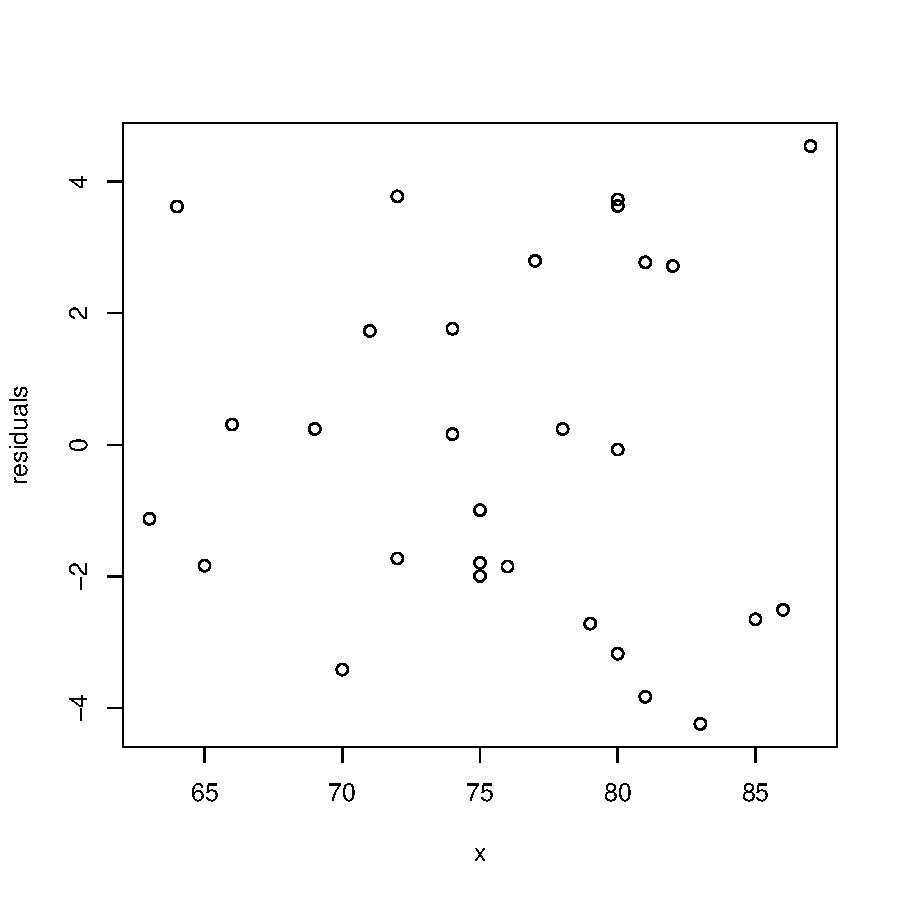
\includegraphics{HW3-025}
\end{figure}
The fluctuations of residuals around zero look uniform and do not seem to be dependent on the predictor. Thus our assumption of homoscedascity in the classical linear model is verified here.

The column rank of the design matrix X can be calculated as:
\begin{Schunk}
\begin{Soutput}
[1] 2
\end{Soutput}
\end{Schunk}
which confirms our assumption of full column rank design matrix.

\clearpage
\begin{itemize}
\item QQ Plot for residuals
\begin{figure}[H]
\begin{Schunk}
\begin{Sinput}
> qqnorm(residuals)
> qqline(residuals)
\end{Sinput}
\end{Schunk}
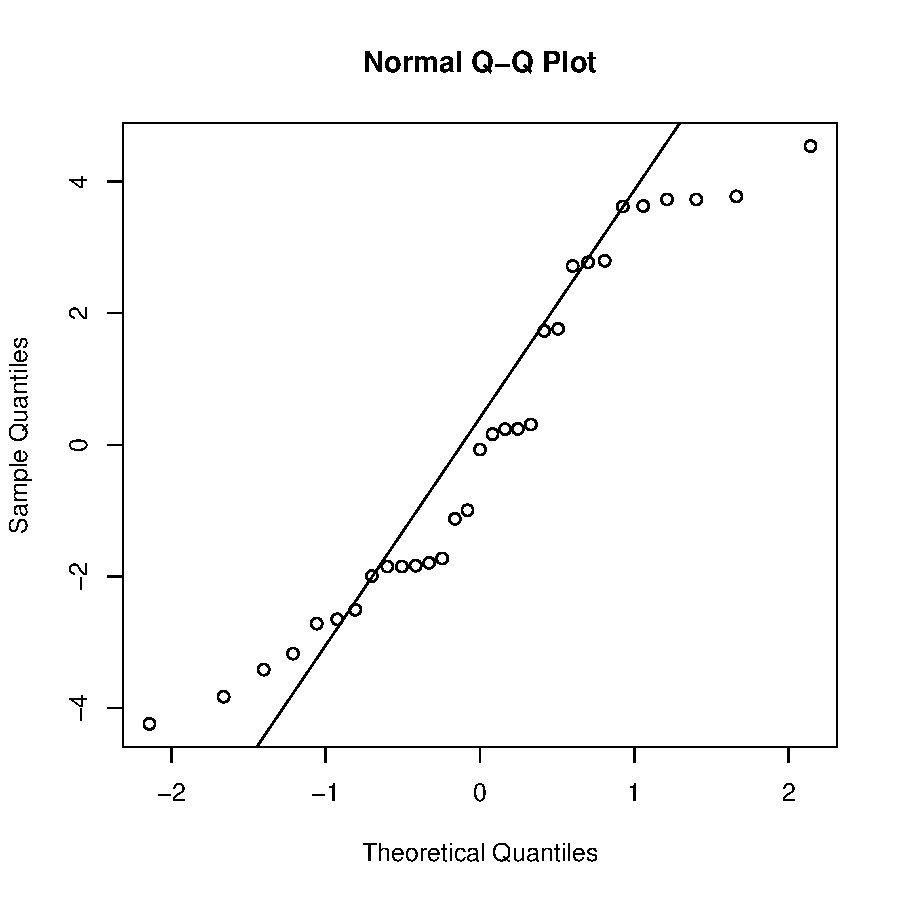
\includegraphics{HW3-027}
\end{figure}
The above QQ plot shows significant deviation from our normality assumption.
\end{itemize}

\item From the scatter plots of various transformations, it seems that there is no transformation that works better than the existing model which suggests that there is no need for modify the model.
\en

\section*{Answer 3}
\bn
\item
\begin{figure}[H]
\begin{Schunk}
\begin{Sinput}
> Munich=read.csv("rent99.raw",sep=" ")
> Munich.rent<-Munich[,c(1,3,4)]
> str(Munich.rent)
\end{Sinput}
\begin{Soutput}
'data.frame':	3082 obs. of  3 variables:
 $ rent : num  121 437 356 283 807 ...
 $ area : int  35 104 29 39 97 62 31 61 72 75 ...
 $ yearc: num  1939 1939 1971 1972 1985 ...
\end{Soutput}
\begin{Sinput}
> pairs(Munich.rent)
> rent<-Munich.rent[,1]
> area<-Munich.rent[,2]
> yearc<-Munich.rent[,3]
> rentsqm<-Munich[,2]
\end{Sinput}
\end{Schunk}
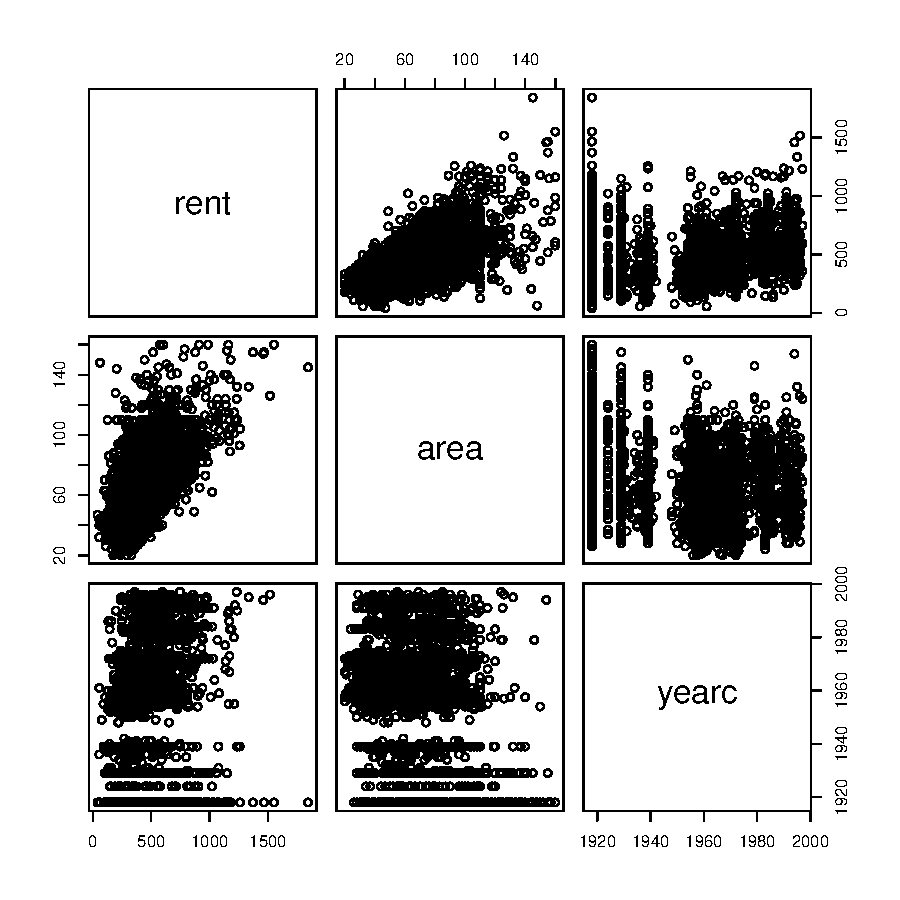
\includegraphics{HW3-028}
\end{figure}
\clearpage

For exploratory data analysis, pairwise scatter plots between the rent, area and yearc variables have been drawn here. The scatter plot between rent and area suggests that as area is increased, the variability of rent increases i.e. for larger area apartments there are more options available in terms of rent, as compared to the smaller area apartments. This is the well known phenomenon of heteroscedascity and will result in the improper estimation of the variances of estimated regression coefficients $\hat{\beta}$. Further, the scatterplots involving yearc variable variable suggests that there are clear cut breaks during the time intervals of 1920-1930 and 1940-1950. The former points out that the data during the period might be extrapolated and therefore not that reliable to analyze while the latter might be accounted by noting that there might be a scarcity of apartments built during World War 2.

\item Fitting the given linear regression model,
\begin{equation*}
\begin{aligned}
rent &= \beta_0 + \beta_1 area + \beta_2 yearc + \epsilon, \hspace{0.1in} \epsilon \sim N(0,\sigma^2)
\end{aligned}
\end{equation*}

\begin{Schunk}
\begin{Sinput}
> fit=lm(rent~area+yearc)
> summary(fit)
\end{Sinput}
\begin{Soutput}
Call:
lm(formula = rent ~ area + yearc)

Residuals:
    Min      1Q  Median      3Q     Max 
-734.76  -94.75  -10.87   82.55 1063.17 

Coefficients:
              Estimate Std. Error t value Pr(>|t|)    
(Intercept) -4775.5942   244.3549  -19.54   <2e-16 ***
area            5.3618     0.1165   46.01   <2e-16 ***
yearc           2.4913     0.1239   20.11   <2e-16 ***
---
Signif. codes:  0 ‘***’ 0.001 ‘**’ 0.01 ‘*’ 0.05 ‘.’ 0.1 ‘ ’ 1 

Residual standard error: 149.3 on 3079 degrees of freedom
Multiple R-squared: 0.4181,	Adjusted R-squared: 0.4177 
F-statistic:  1106 on 2 and 3079 DF,  p-value: < 2.2e-16 
\end{Soutput}
\end{Schunk}

The summary of the model fitted shows the estimated values of the parameters and the various quantiles for residuals. Further the mean of the residuals vector is calculated as 
\begin{Schunk}
\begin{Sinput}
> residuals=fit$resid
> mean(residuals)
\end{Sinput}
\begin{Soutput}
[1] -4.664461e-15
\end{Soutput}
\end{Schunk}
which is very close to zero, thus verifying our assumption of $E(\epsilon)=0$. The column rank of the design matrix X can be calculated as:
\begin{Schunk}
\begin{Soutput}
[1] 3
\end{Soutput}
\end{Schunk}
which confirms our assumption of full column rank design matrix.
The relevant plots after fitting the model and their interpretations are given as follows:
\begin{itemize}
\item Plot of model residuals vs. fitted values:
\begin{figure}[H]
\begin{Schunk}
\begin{Sinput}
> yhat=fit$fitted.values
> plot(yhat,residuals)
\end{Sinput}
\end{Schunk}
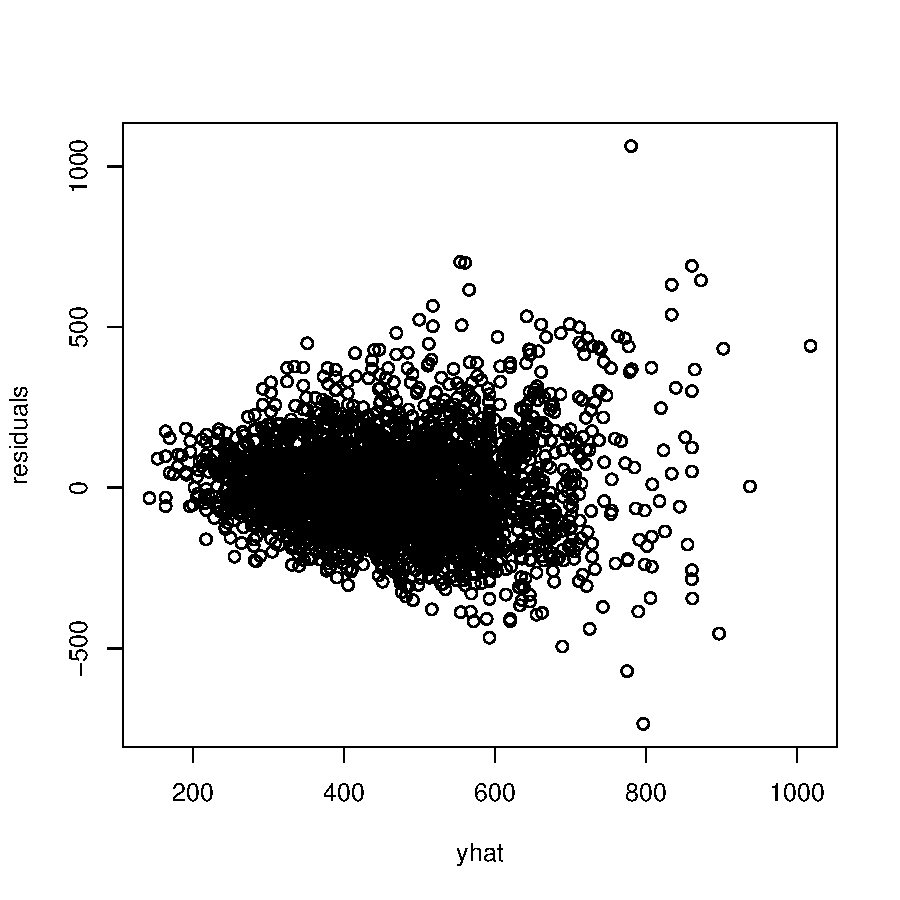
\includegraphics{HW3-032}
\end{figure}
The funnel shaped behaviour of the above residual plot indicates increase in variance of the residuals with the fitted values (or the covariates) which implies heteroscedascity. Thus here the assumption of homoscedascity in our classical linear model is violated.
\clearpage

\item Partial residual plot for area
\begin{figure}[H]
\begin{Schunk}
\begin{Sinput}
> beta=fit$coef
> p.residuals.area=residuals+beta[2]*area
> plot(area,p.residuals.area)
\end{Sinput}
\end{Schunk}
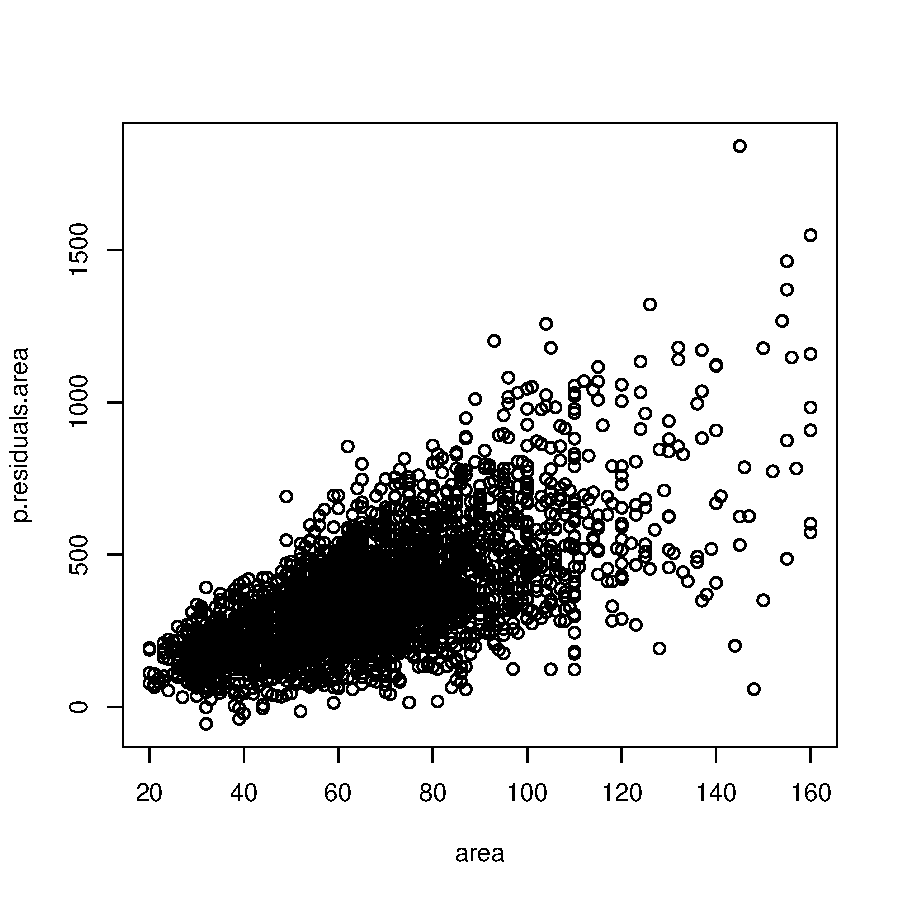
\includegraphics{HW3-033}
\end{figure}
\clearpage

The above partial residual plot of area shows that the variance of rent increases as the area is increased. Further the points are much more separated towards larger areas which shows that there are lesser options in terms of choosing rent values from a particular interval for larger area apartments.  

\item Partial residual plot for yearc
\begin{figure}[H]
\begin{Schunk}
\begin{Sinput}
> p.residuals.yearc=residuals+beta[3]*yearc
> plot(yearc,p.residuals.yearc)
\end{Sinput}
\end{Schunk}
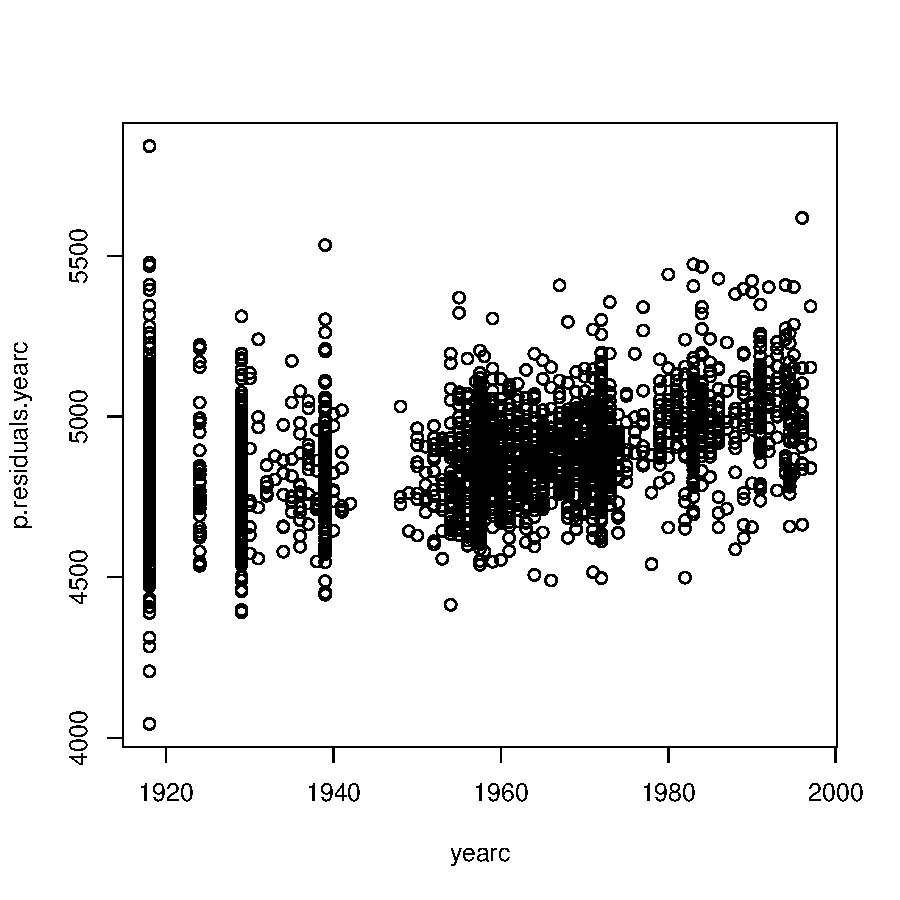
\includegraphics{HW3-034}
\end{figure}
\clearpage

The above partial residual plot of yearc shows that there are blank spaces approximately in the intervals 1920-1930 and 1940-1950 which shows that the number of houses constructed during this period was much smaller.

\item QQ Plot for residuals
\begin{figure}[H]
\begin{Schunk}
\begin{Sinput}
> qqnorm(residuals)
> qqline(residuals)
\end{Sinput}
\end{Schunk}
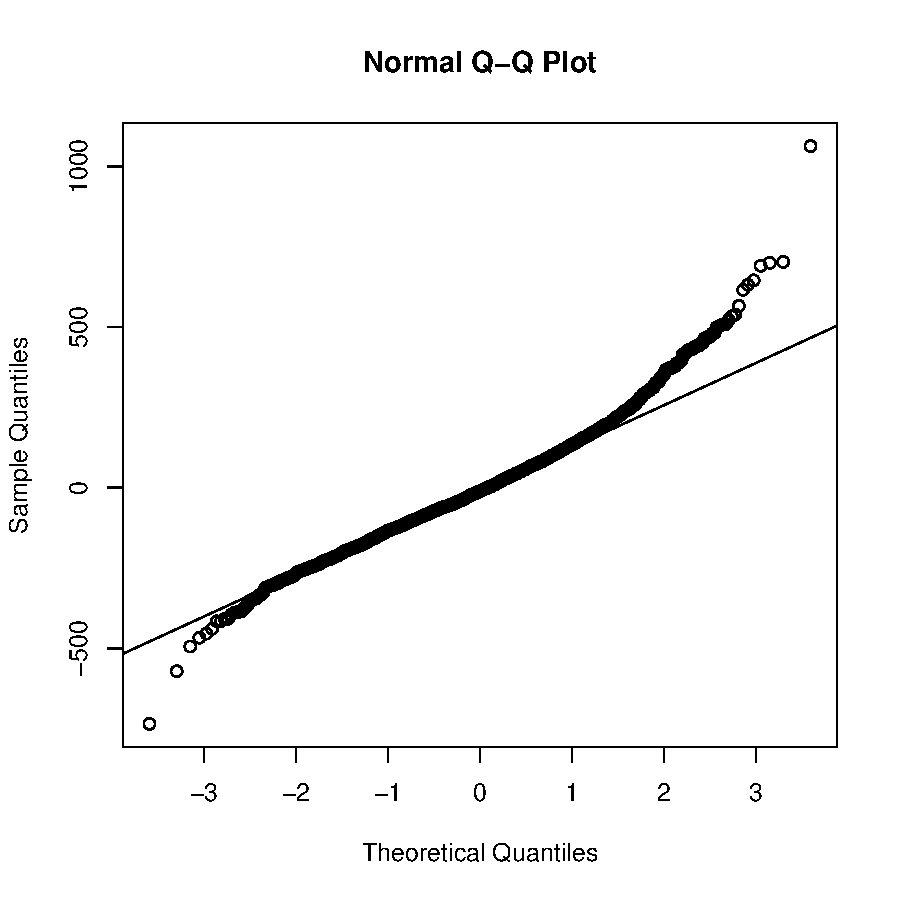
\includegraphics{HW3-035}
\end{figure}
The fat tails on both the ends clearly indicates deviation from our normality assumption.
\end{itemize}
%--------------------------------------------------------------------------------------
% part (c) and (d)
\item Now fitting the model 
\begin{equation*}
\begin{aligned}
log(rent) &= \beta_0 + \beta_1 area + \beta_2 yearc + \epsilon, \epsilon \sim N(0,\sigma^2)
\end{aligned}
\end{equation*}

\begin{Schunk}
\begin{Sinput}
> lrent<-log(rent)
> fit<-lm(lrent~area+yearc)
> summary(fit)
\end{Sinput}
\begin{Soutput}
Call:
lm(formula = lrent ~ area + yearc)

Residuals:
    Min      1Q  Median      3Q     Max 
-2.5900 -0.1890  0.0236  0.2213  0.9213 

Coefficients:
              Estimate Std. Error t value Pr(>|t|)    
(Intercept) -6.6385556  0.5446836  -12.19   <2e-16 ***
area         0.0111738  0.0002598   43.01   <2e-16 ***
yearc        0.0060972  0.0002762   22.07   <2e-16 ***
---
Signif. codes:  0 ‘***’ 0.001 ‘**’ 0.01 ‘*’ 0.05 ‘.’ 0.1 ‘ ’ 1 

Residual standard error: 0.3328 on 3079 degrees of freedom
Multiple R-squared: 0.3945,	Adjusted R-squared: 0.3941 
F-statistic:  1003 on 2 and 3079 DF,  p-value: < 2.2e-16 
\end{Soutput}
\end{Schunk}

The summary of the model fitted shows the estimated values of the parameters and the various quantiles for residuals. 

\item The mean of the residuals vector is calculated as 
\begin{Schunk}
\begin{Sinput}
> residuals=fit$resid
> mean(residuals)
\end{Sinput}
\begin{Soutput}
[1] 1.342919e-17
\end{Soutput}
\end{Schunk}
which is very close to zero, thus verifying our assumption of $E(\epsilon)=0$. The column rank of the design matrix X can be calculated as:
\begin{Schunk}
\begin{Soutput}
[1] 3
\end{Soutput}
\end{Schunk}
which confirms our assumption of full column rank design matrix.
The relevant plots after fitting the model and their interpretations are given as follows:
\clearpage
\begin{itemize}
\item Plot of model residuals vs. fitted values:
\begin{figure}[H]
\begin{Schunk}
\begin{Sinput}
> yhat<-fit$fitted.values
> plot(yhat,residuals)
\end{Sinput}
\end{Schunk}
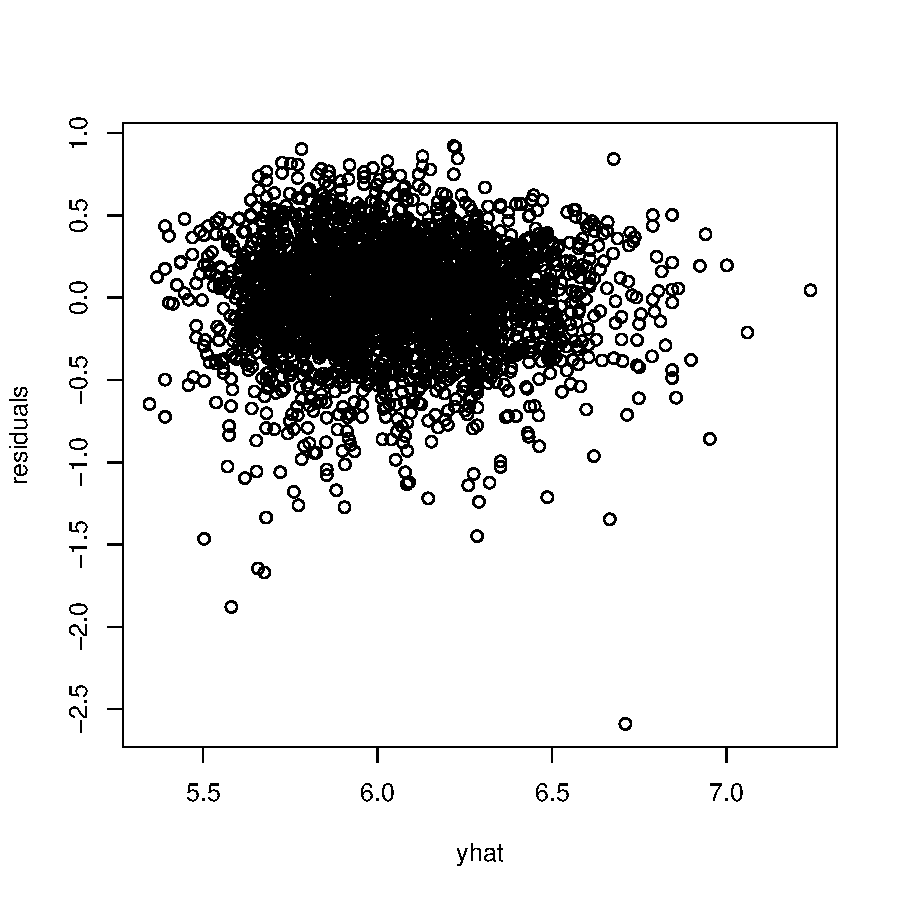
\includegraphics{HW3-039}
\end{figure}
The above residual plot is much better than the previous one. However still there are some points that go as down as -2. Further the density of points towards the right is also smaller. But rest of the points are fairly uniformly distributed and thus we can say that our assumption of homoscedascity is approximately satisfied here.

\clearpage

\item Partial residual plot for area
\begin{figure}[H]
\begin{Schunk}
\begin{Sinput}
> beta<-fit$coef
> p.residuals.area<-residuals+beta[2]*area
> plot(area,p.residuals.area)
\end{Sinput}
\end{Schunk}
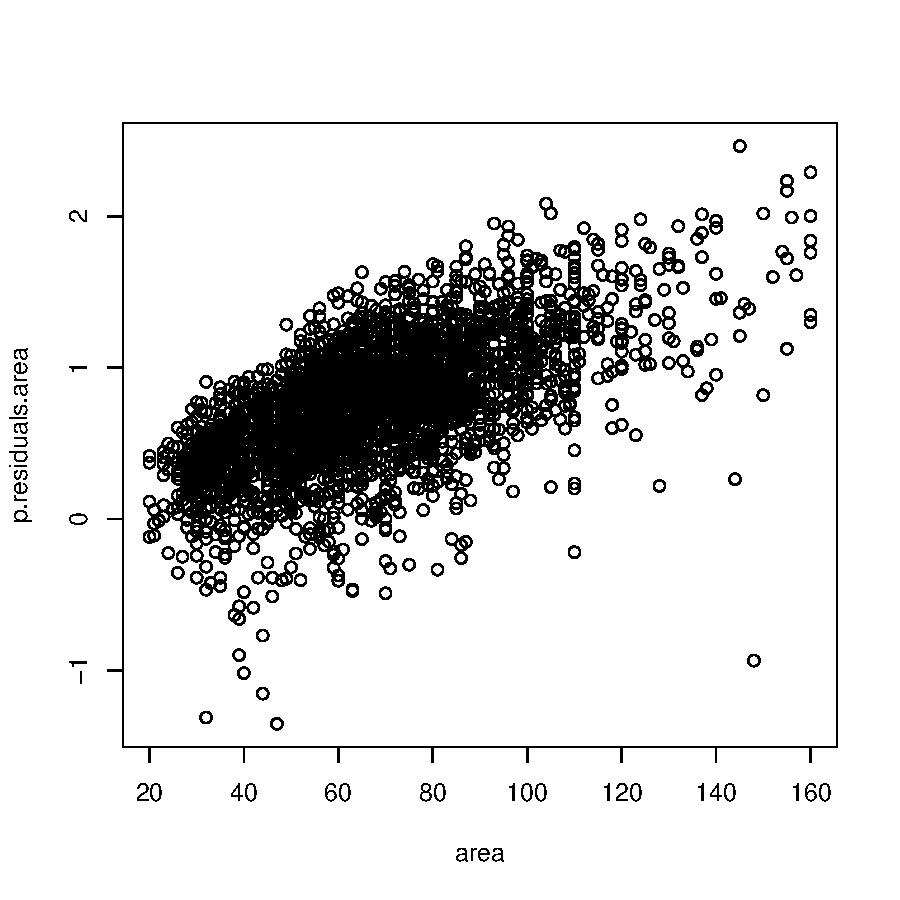
\includegraphics{HW3-040}
\end{figure}
\clearpage

The above partial residual plot indicates that unlike the previous one, the variance of log of rent does not vary with area. and follows a linear relationship.

\item Partial residual plot for yearc
\begin{figure}[H]
\begin{Schunk}
\begin{Sinput}
> p.residuals.yearc<-residuals+beta[3]*yearc
> plot(yearc,p.residuals.yearc)
\end{Sinput}
\end{Schunk}
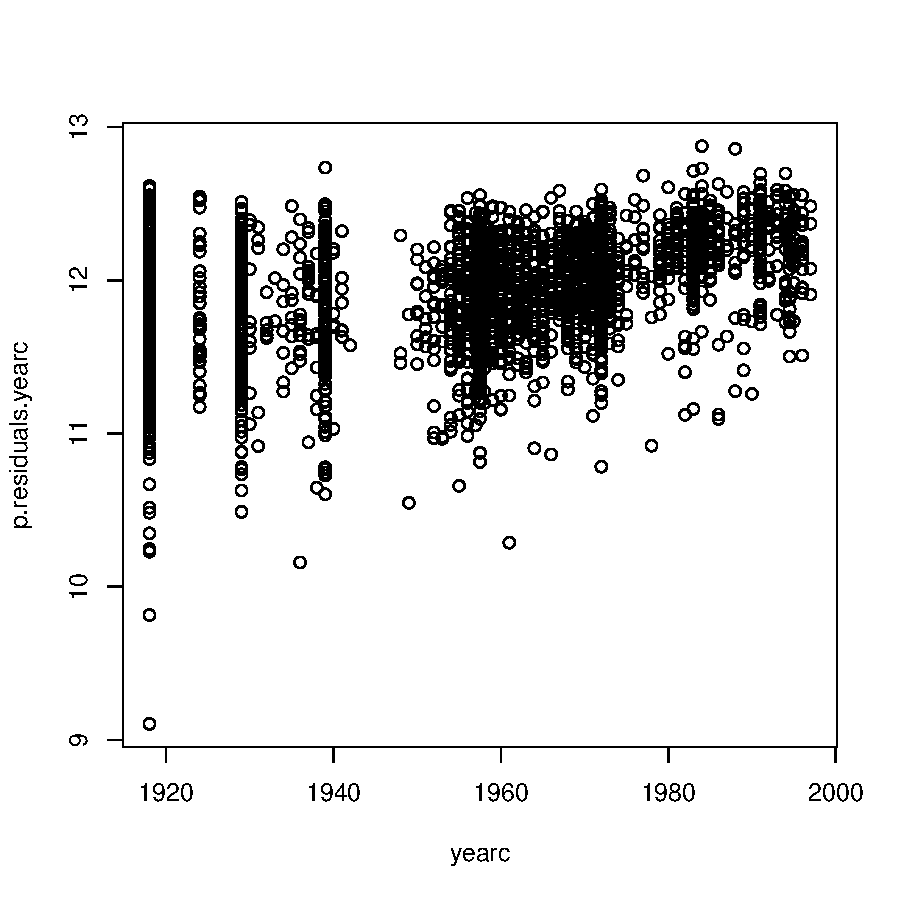
\includegraphics{HW3-041}
\end{figure}
\clearpage

The above residual plot again clearly shows missing data points in the intervals 1920-1925 and 1940-1950 which indicates that there were not many apartments that were constructed during these periods. 

\item QQ Plot for residuals
\begin{figure}[H]
\begin{Schunk}
\begin{Sinput}
> qqnorm(residuals)
> qqline(residuals)
\end{Sinput}
\end{Schunk}
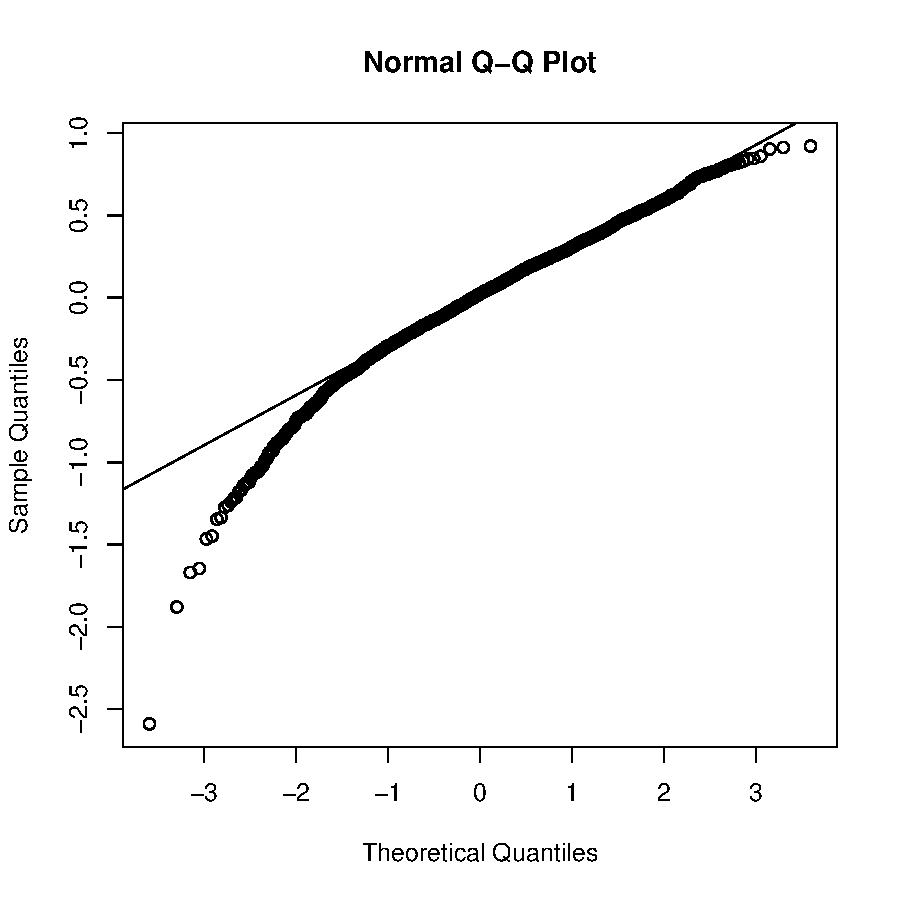
\includegraphics{HW3-042}
\end{figure}
The fat tail on the left end and less prominent short tail on the right end clearly indicates significant deviation from our normality assumption.
\end{itemize}

%------------------------------------------------------------------------------------
% part (e)

\item  Now fitting the model 
\begin{equation*}
\begin{aligned}
rentsqm &= \beta_0 + \beta_1 area + \beta_2 yearc + \epsilon, \hspace{0.1in} \epsilon \sim N(0,\sigma^2)
\end{aligned}
\end{equation*}

%\begin{figure}[H]
\begin{Schunk}
\begin{Sinput}
> fit<-lm(rentsqm~area+yearc)
> #par (mfrow=c(2,2))
> #plot(fit,which=1:4)
> summary(fit)
\end{Sinput}
\begin{Soutput}
Call:
lm(formula = rentsqm ~ area + yearc)

Residuals:
    Min      1Q  Median      3Q     Max 
-6.5261 -1.5604 -0.1481  1.4134  9.0863 

Coefficients:
              Estimate Std. Error t value Pr(>|t|)    
(Intercept) -61.058133   3.527255  -17.31   <2e-16 ***
area         -0.027231   0.001682  -16.19   <2e-16 ***
yearc         0.035784   0.001789   20.01   <2e-16 ***
---
Signif. codes:  0 ‘***’ 0.001 ‘**’ 0.01 ‘*’ 0.05 ‘.’ 0.1 ‘ ’ 1 

Residual standard error: 2.155 on 3079 degrees of freedom
Multiple R-squared: 0.2178,	Adjusted R-squared: 0.2173 
F-statistic: 428.6 on 2 and 3079 DF,  p-value: < 2.2e-16 
\end{Soutput}
\end{Schunk}
%\end{figure}

The summary of the model fitted shows the estimated values of the parameters and the various quantiles for residuals. 

The mean of the residuals vector is calculated as 
\begin{Schunk}
\begin{Sinput}
> residuals<-fit$resid
> mean(residuals)
\end{Sinput}
\begin{Soutput}
[1] -1.58401e-16
\end{Soutput}
\end{Schunk}
which is very close to zero, thus verifying our assumption of $E(\epsilon)=0$. The design matrix is same as last part and satisfies the full rank assumption. The relevant plots after fitting the model and their interpretations are given as follows:
\clearpage
\begin{itemize}
\item Plot of model residuals vs. fitted values:
\begin{figure}[H]
\begin{Schunk}
\begin{Sinput}
> yhat<-fit$fitted.values
> plot(yhat,residuals)
\end{Sinput}
\end{Schunk}
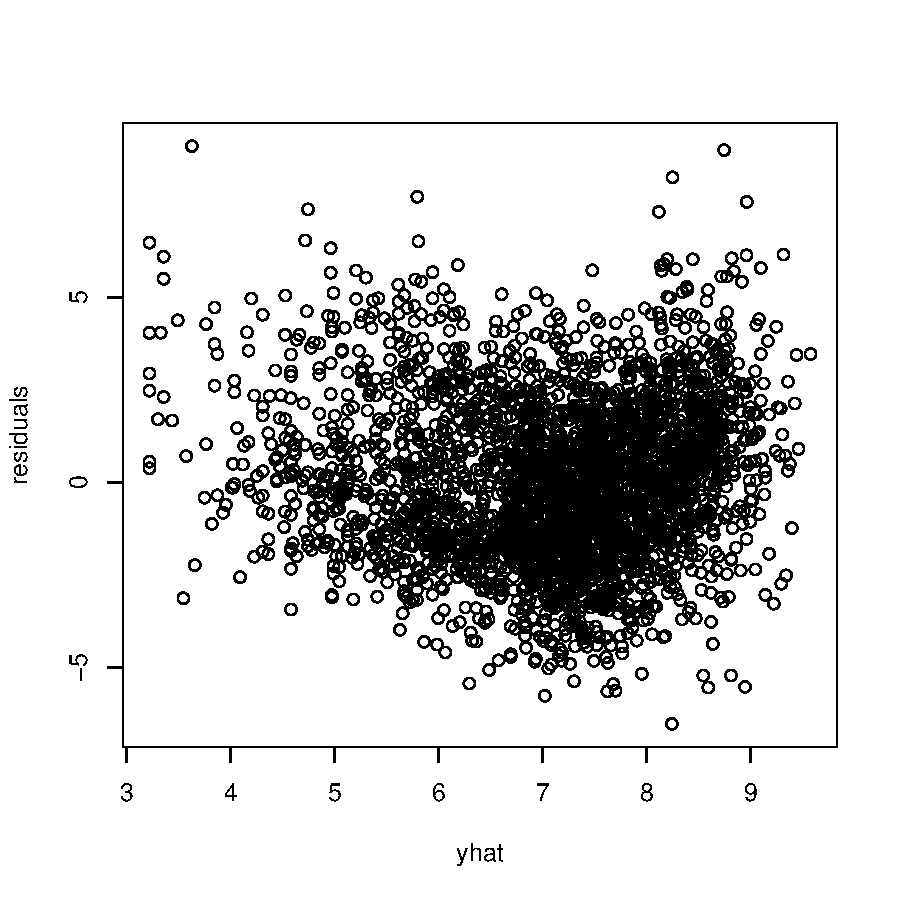
\includegraphics{HW3-045}
\end{figure}
The above residual plot shows residuals are much more uniformly distributed compared to the last two models. Thus our assumption of homoscdascity is approximately satisfied here.
\clearpage

\item Partial residual plot for area
\begin{figure}[H]
\begin{Schunk}
\begin{Sinput}
> beta<-fit$coef
> p.residuals.area<-residuals+beta[2]*area
> plot(area,p.residuals.area)
\end{Sinput}
\end{Schunk}
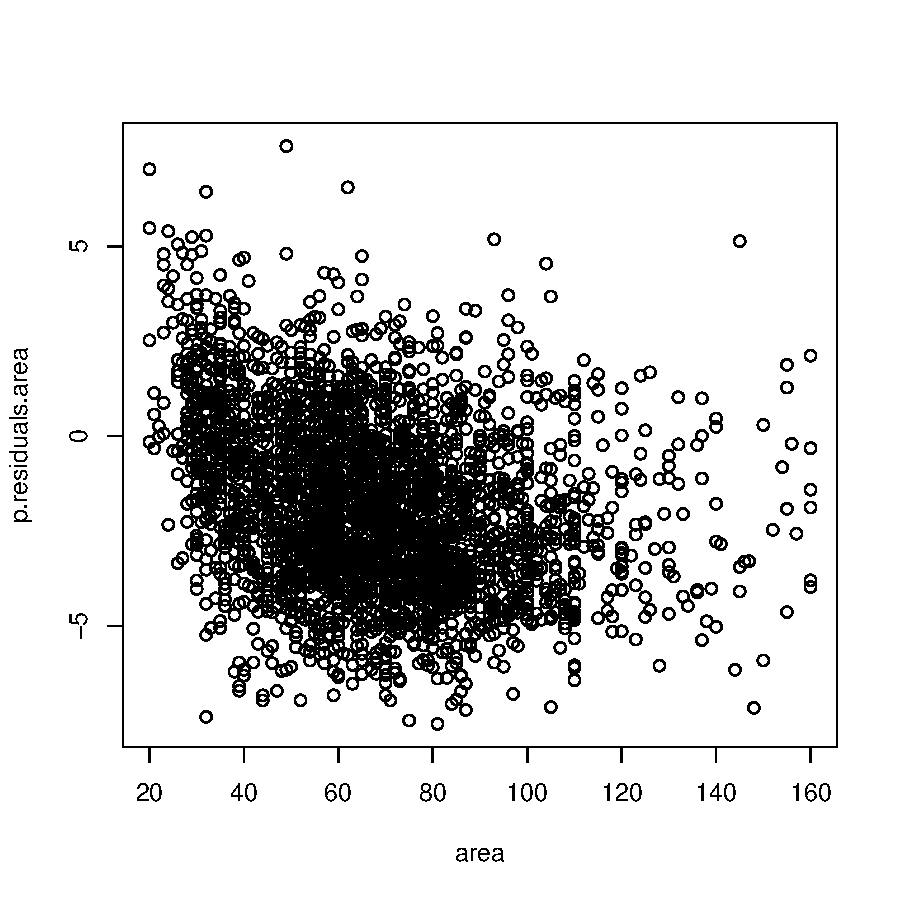
\includegraphics{HW3-046}
\end{figure}
\clearpage

\item Partial residual plot for yearc
\begin{figure}[H]
\begin{Schunk}
\begin{Sinput}
> p.residuals.yearc<-residuals+beta[3]*yearc
> plot(yearc,p.residuals.yearc)
\end{Sinput}
\end{Schunk}
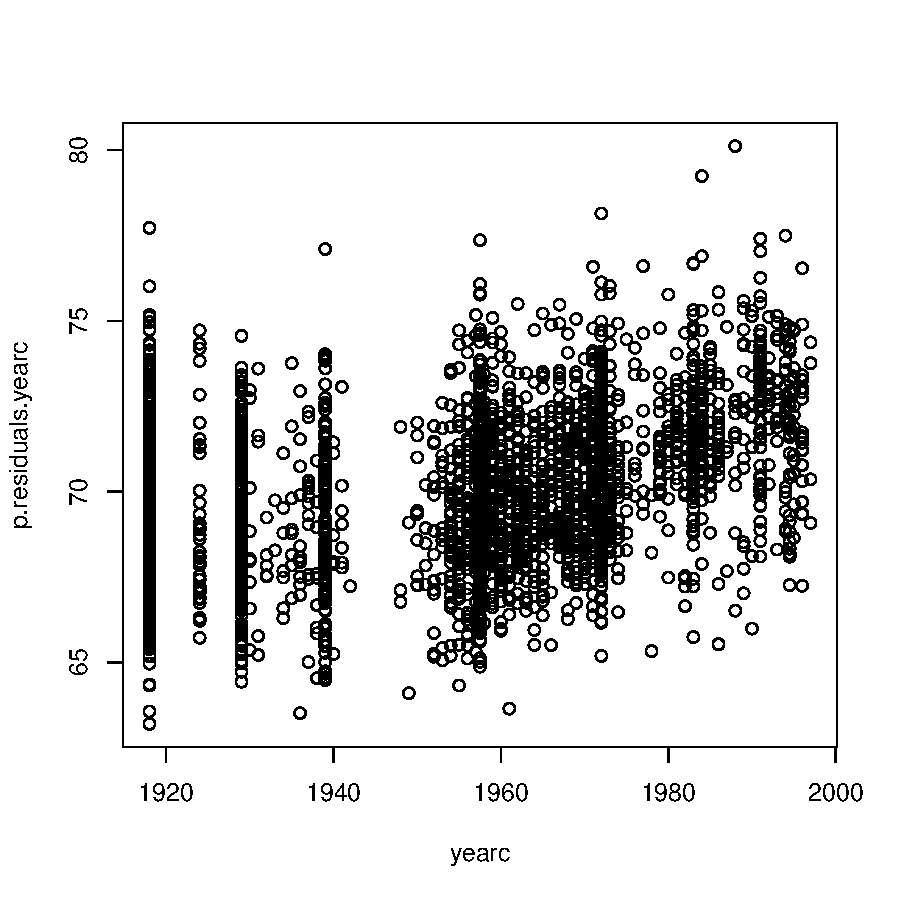
\includegraphics{HW3-047}
\end{figure}
\clearpage

\item QQ Plot for residuals
\begin{figure}[H]
\begin{Schunk}
\begin{Sinput}
> qqnorm(residuals)
> qqline(residuals)
\end{Sinput}
\end{Schunk}
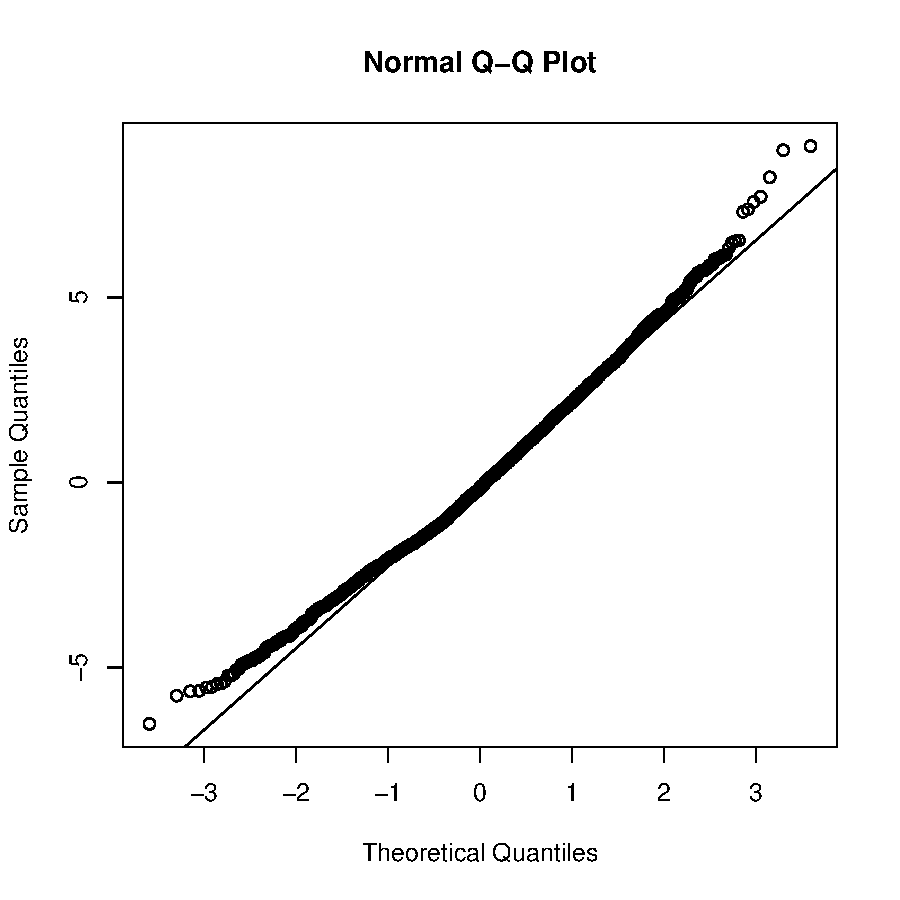
\includegraphics{HW3-048}
\end{figure}
The short tail towards the left end and a fat tail towards the right end indicates a very slight deviation from our normality assumption. This is much better than our earlier models.
\end{itemize}

%---------------------------------------------------------------------------------
% part (f)
\item
Choosing $f(area)=\beta_1 \dfrac{1}{area}$ and $g(yearc)=\beta_2 yearc + \beta_2 yearc^2 + \beta_3 yearc^3$, we obtain the model as
\begin{equation*}
\begin{aligned}
rentsqm &= \beta_0 + \beta_1 \dfrac{1}{area} + \beta_2 yearc + \beta_3 yearc^2 + \beta_4 yearc^3 + \epsilon, \hspace{0.1in} \epsilon \sim N(0,\sigma^2)
\end{aligned}
\end{equation*}

Fitting this model we get:
%\begin{figure}[H]
\begin{Schunk}
\begin{Sinput}
> fit3.4<-lm(rentsqm~I(1/area)+poly(yearc,3))
> #par (mfrow=c(2,2))
> #plot(fit,which=1:4)
> summary(fit3.4)
\end{Sinput}
\begin{Soutput}
Call:
lm(formula = rentsqm ~ I(1/area) + poly(yearc, 3))

Residuals:
    Min      1Q  Median      3Q     Max 
-6.9920 -1.3705 -0.1354  1.3711  8.2834 

Coefficients:
                Estimate Std. Error t value Pr(>|t|)    
(Intercept)       4.9121     0.1009  48.692   <2e-16 ***
I(1/area)       129.5717     5.5358  23.406   <2e-16 ***
poly(yearc, 3)1  43.9384     2.0726  21.200   <2e-16 ***
poly(yearc, 3)2  27.5389     2.0596  13.371   <2e-16 ***
poly(yearc, 3)3  -1.7558     2.0400  -0.861    0.389    
---
Signif. codes:  0 ‘***’ 0.001 ‘**’ 0.01 ‘*’ 0.05 ‘.’ 0.1 ‘ ’ 1 

Residual standard error: 2.039 on 3077 degrees of freedom
Multiple R-squared:   0.3,	Adjusted R-squared: 0.2991 
F-statistic: 329.7 on 4 and 3077 DF,  p-value: < 2.2e-16 
\end{Soutput}
\end{Schunk}
%\end{figure}

The summary of the model fitted shows the estimated values of the parameters and the various quantiles for residuals. 

The mean of the residuals vector is calculated as 
\begin{Schunk}
\begin{Sinput}
> residuals3.4<-fit3.4$resid
> mean(residuals3.4)
\end{Sinput}
\begin{Soutput}
[1] 1.90071e-17
\end{Soutput}
\end{Schunk}
which is very close to zero, thus verifying our assumption of $E(\epsilon)=0$. The column rank of the design matrix X can be calculated as:
\begin{Schunk}
\begin{Soutput}
[1] 5
\end{Soutput}
\end{Schunk}
which confirms our assumption of full column rank design matrix.
The relevant plots after fitting the model and their interpretations are given as follows:
\clearpage
\begin{itemize}
\item Plot of model residuals vs. fitted values:
\begin{figure}[H]
\begin{Schunk}
\begin{Sinput}
> yhat3.4<-fit3.4$fitted.values
> plot(yhat3.4,residuals3.4)
\end{Sinput}
\end{Schunk}
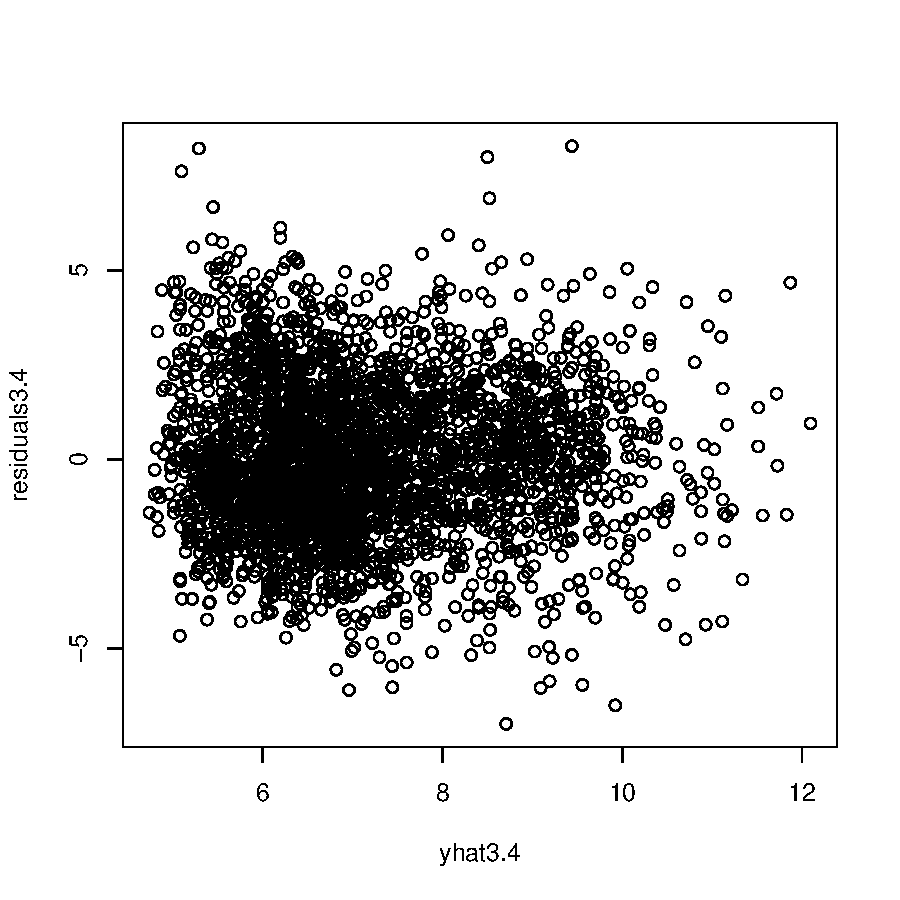
\includegraphics{HW3-052}
\end{figure}
The above residual plot shows residuals are much more uniformly distributed compared to the last three models. Thus our assumption of homoscdascity is satisfied here to a great extent.
\clearpage

\item Partial residual plots for area and yearc
\begin{figure}[H]
\begin{Schunk}
\begin{Sinput}
> library(car)
> crPlots(fit3.4)
\end{Sinput}
\end{Schunk}
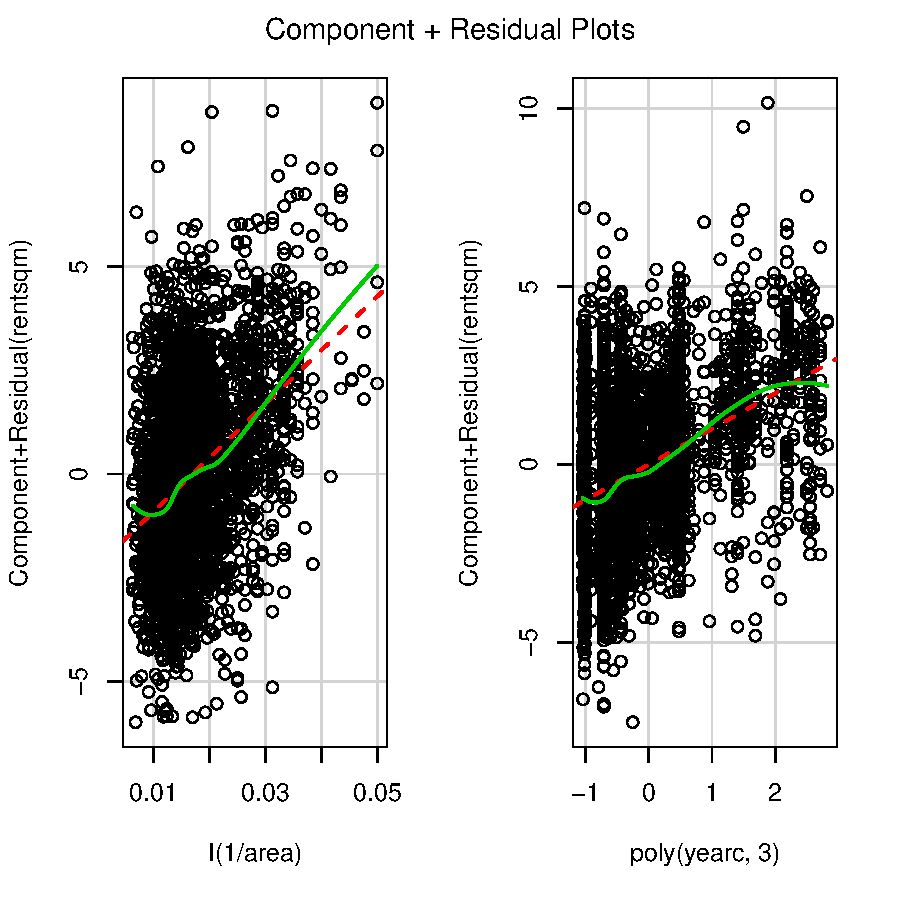
\includegraphics{HW3-053}
\end{figure}
\clearpage

From the partial residual plot of rentsqm vs. area, it is clear that as area is increased the variability in rent per square meter increases. For a smaller area apartment, the number of options in terms of rent per square meter are densely concentrated in smaller intervals while for a larger area apartment they span a much larger interval but are sparsely distributed. Further, the partial residual plot of rentsqm vs. yearc again shows an increasing trend of rent per square meter as time of construction (in years) passes. Notably there are a few spots in the middle where the number of options in terms of rent per square meter are much lesser, indicating a decrease in the construction of number of houses during that particular period.  

\item QQ Plot for residuals
\begin{figure}[H]
\begin{Schunk}
\begin{Sinput}
> qqnorm(residuals3.4)
> qqline(residuals3.4)
\end{Sinput}
\end{Schunk}
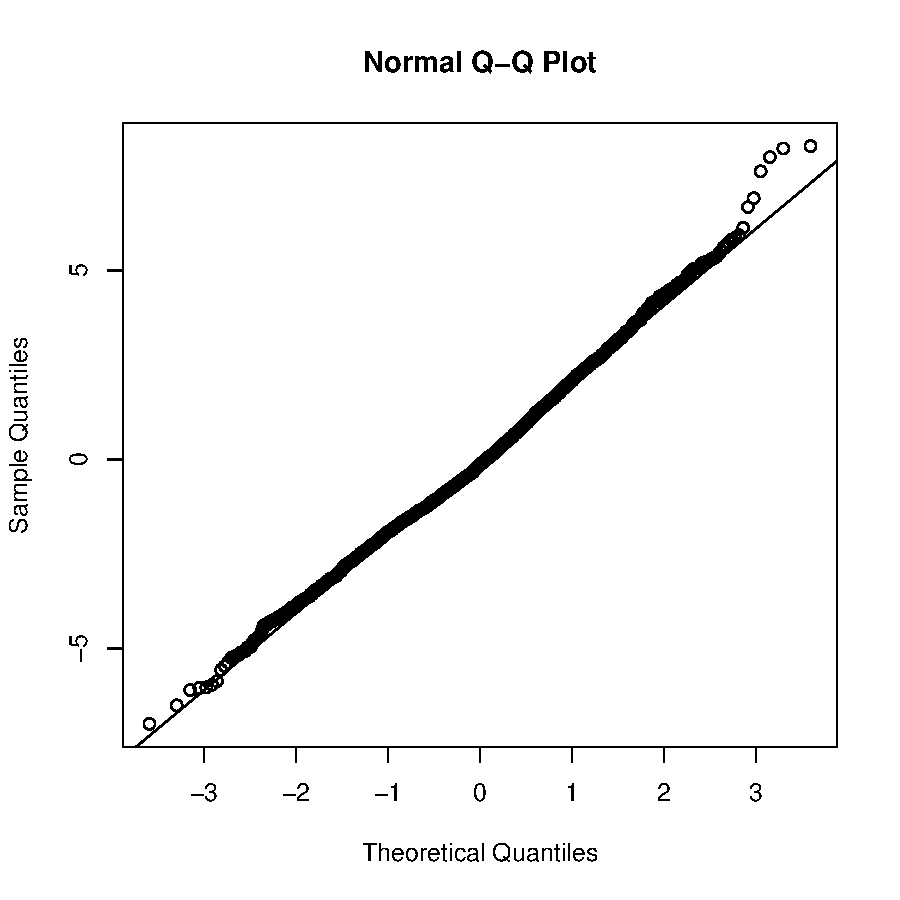
\includegraphics{HW3-054}
\end{figure}
The small fat tail towards the right end indicates a very slight deviation from our normality assumption.
\end{itemize}

\item Multiplying the finalized model in part (f) by area and taking the expectation, we get,

$rentsqm \times area = \beta_0 \times area + \beta_1 \dfrac{1}{area} \times area + \beta_2 yearc \times area + \beta_3 yearc^2 \times area  + \beta_4 yearc^3 \times area + \epsilon \times area, \hspace{0.1in} \epsilon \sim N(0,\sigma^2)$

which simplifies as\\
$rent = \beta_0 \times area + \beta_1 + \beta_2 yearc \times area + \beta_3 yearc^2 \times area  + \beta_4 yearc^3 \times area + \epsilon \times area, \hspace{0.1in} \epsilon \sim N(0,\sigma^2)$

The estimated expected rent thus becomes\\
E[$\widehat{rent}] = \hat{\beta_0} \times area + \hat{\beta_1} + \hat{\beta_2} yearc \times area + \hat{\beta_3} yearc^2 \times area  + \hat{\beta_4} yearc^3 \times area + E[\widehat{\epsilon}] \times area, \hspace{0.1in} \epsilon \sim N(0,\sigma^2)$

Now $E[\hat{\epsilon}]=0$. Thus we obtain\\
$\widehat{E[rent]} = \hat{\beta_0} \times area + \hat{\beta_1} + \hat{\beta_2} yearc \times area + \hat{\beta_3} yearc^2 \times area  + \hat{\beta_4} yearc^3 \times area$

The interaction terms of the area and yearc covariates clearly indicates that the rate of increase of rent with an unit increase in area is higher for a later time period as compared to an earlier time period. The estimated parameter values are already shown in the summary before.

The variance of rent can be calculated as\\

\begin{equation*}
\begin{aligned}
Var[\widehat{rent}] &= Var[\hat{\epsilon}] \times area^2, \hspace{0.1in} \epsilon \sim N(0,\sigma^2)\\
&= \widehat{\sigma^2} \times area^2
\end{aligned}
\end{equation*}

It is clear from the above expression that there is no effect of yearc on the variance of rent. However the variance of rent is proprtional to the square of area.

\item Following models were tried before finalizing this particular model. 
\begin{itemize}

\item
\begin{equation*}
\begin{aligned}
rentsqm &= \beta_0 + \beta_1 \dfrac{1}{area} + \beta_2 yearc + \epsilon, \hspace{0.1in} \epsilon \sim N(0,\sigma^2)
\end{aligned}
\end{equation*}

\item
\begin{equation*}
\begin{aligned}
rentsqm &= \beta_0 + \beta_1 \dfrac{1}{area^2} + \beta_2 yearc^2 + \epsilon, \hspace{0.1in} \epsilon \sim N(0,\sigma^2)
\end{aligned}
\end{equation*}

\item
\begin{equation*}
\begin{aligned}
rentsqm &= \beta_0 + \beta_1 log(area) + \beta_2 yearc +\beta_3 yearc^2 + \epsilon, \hspace{0.1in} \epsilon \sim N(0,\sigma^2)
\end{aligned}
\end{equation*}

\end{itemize}

There were one or more of the following major problems with the above models:

\begin{itemize}
\item Our assumption of homoscedascity was not satisfied (visually inferred from the residual plots)
\item Our assumption of normal errors was not satisfied (visually inferred from QQ plot)
\item The partial residual plots were bizzare.
\end{itemize}

If I were to choose one of these I would choose the first one since it most closely satisfies our assumptions of homoscedascity and normality under the classical linear model.
\en
\end{document}
